\documentclass[pdftex, a4paper, oneside, parskip, numbers=noenddot, listof=totoc, bibliography=totocnumbered, hyperfootnotes=false]{scrreprt}

%%%%%%%%%%%%%%%%%%%%%%%%%%%%%%%%%%Imports%%%%%%%%%%%%%%%%%%%%%%%%%%%%%%%%%%%%%%

% geometry
\usepackage[bindingoffset=1cm, left=2.5cm, right=2.5cm, top=2.5cm, bottom=2.5cm]{geometry}

% Headline
\usepackage{fancyhdr}

% Select input encodung, usually utf8 is the best choice, on windows, \usepackage[latin1]{inputenc} maybe required
\usepackage[utf8]{inputenc}
\usepackage[T1]{fontenc}

% Colors
\usepackage{color}
\usepackage{colortbl}

% Tables
\usepackage{tabularx}
\usepackage{multirow}

% Drawing graphs etc.
\usepackage{pgf}
\usepackage{tikz}
\usetikzlibrary{arrows,automata}

% math
\usepackage{amsmath} 

% lists
\usepackage{paralist}

% Figures
\usepackage{graphicx, wrapfig}
\usepackage{subfig}

% Hyperlinks
\usepackage[hyphens]{url}
\usepackage{hyperref}

% Listings
\usepackage[outputdir=out]{minted}

% list of abbreviations
\usepackage[printonlyused]{acronym}

% Set line pitch
\usepackage{setspace}

% Figures
\usepackage{caption}
\usepackage[hypcap=true,labelformat=simple]{subcaption}

% Tables
\usepackage{booktabs} 


\usepackage[backend=biber,style=alphabetic,sorting=ynt]{biblatex}

\usepackage{csquotes}

%%%%%%%%%%%%%%%%%%%%%%%%%%%%%%%%%%%%%%%%%%%%%%%%%%%%%%%%%%%%%%%%%%%%%%%%%%%%%%%

\pagestyle{fancy}
\renewcommand{\chaptermark}[1]{\markboth{\thechapter\ #1}{}}
\newcommand{\chaptermarker}[1]{\markboth{#1}{}}
\lhead{\leftmark} \rhead{\thepage}
\cfoot{}
\fancypagestyle{plain}{}

\setcounter{secnumdepth}{\subsubsectionnumdepth}

\usetikzlibrary{arrows,automata}

\hypersetup{colorlinks, citecolor=black, linkcolor=black, urlcolor=black}

\onehalfspacing

% Layout corrections (Schusterjungen)
\clubpenalty = 10000
% Layout corrections (Hurenkinder) 
\widowpenalty = 10000
\displaywidowpenalty = 10000

\renewcommand{\thesubfigure}{(\alph{subfigure})}

% Frequently used column types
\newcolumntype{C}[1]{>{\centering\arraybackslash}p{#1}} % centering column type with fixed width
\newcolumntype{R}[1]{>{\raggedleft\arraybackslash}p{#1}} % right aligned column type with fixed width
\newcolumntype{L}[1]{>{\raggedright\arraybackslash}p{#1}} % left aligned column type with fixed width

\setminted{
    xleftmargin=20pt,
    frame=lines,
    framesep=2mm,
    baselinestretch=1.2,
    fontsize=\footnotesize,
    linenos,
    breaklines,
    escapeinside=``
}

% Proper linebreaks for long urls
\setcounter{biburllcpenalty}{7000}
\setcounter{biburlucpenalty}{8000}

%%%%%%%%%%%%%%%%%%%%%%%%%%%%%%%%%%THESIS%%%%%%%%%%%%%%%%%%%%%%%%%%%%%%%%%%%%%

\newcommand{\thesistitle}{TITEL}
\newcommand{\thesistype}{B A C H E L O R A R B E I T}
\newcommand{\thesistypedesc}{zur Erlangung des Grades eines Bachelor of Science \\im Fachbereich Elektrotechnik/Informatik \\der Universit\"at Kassel}
\newcommand{\thesisauthorname}{VORNAME NACHNAME}
\newcommand{\thesisauthorhomestreet}{STRASSE}
\newcommand{\thesisauthorhometown}{STADT}
\newcommand{\thesisauthormatrikelnumber}{MARTIKELNUMMER}
\newcommand{\thesisauthoremail}{MAIL}
\newcommand{\thesisdepartment}{Fachgebiet Software Engineering}
\newcommand{\thesisfirstreviewer}{!ERSTPR\"UFER! TITEL VORNAME NACHNAME}
\newcommand{\thesissecondreviewer}{!ZWEITPR\"UFER! TITEL VORNAME NACHNAME}
\newcommand{\thesissupervisor}{TITEL VORNAME NACHNAME}
\newcommand{\thesisdate}{\today}

%%%%%%%%%%%%%%%%%%%%%%%%%%%%%%%%%%FLOATS%%%%%%%%%%%%%%%%%%%%%%%%%%%%%%%%%%%%%

% Shortcuts for referencing floats:
\newcommand{\fig}[1]{\figurename~\ref{#1}} %shortcut for a figure reference
\newcommand{\tab}[1]{Table~\ref{#1}} %shortcut for a table reference
\newcommand{\eq}[1]{(\ref{#1})} %shortcut for an equation reference
\newcommand{\lst}[1]{Listing~\ref{#1}} %shortcut for a listing reference
\newcommand{\sect}[1]{Section~\ref{#1}} %shortcut for a Section reference

% Newcommand TODO (red in text)
\newcommand{\todo}[1]{\textcolor{red}{TODO: #1}}

% Newcommand TODOM (red at border)
\newcommand{\todom}[1]{\marginpar{\parbox{1.5cm}{\textcolor{red}{TODO:\\ #1}}}}

\usepackage[ngerman]{babel}
\usepackage{siunitx}
\usepackage{xcolor}

\addbibresource{references.bib}


%%%%%%%%%%%%%%%%%%%%%%%%%%%%%%%%%%DOCUMENT%%%%%%%%%%%%%%%%%%%%%%%%%%%%%%%%%%%%%

\begin{document}
\begin{titlepage}
  %select font without serifs
  \sffamily

  % Logo
  \begin{tabularx}{\textwidth}{@{}l@{}>{\raggedleft\arraybackslash}X@{}r@{}}
    \multirow{2}{*}{
\includegraphics[width=6.8cm]{images/Logo_UniKassel}} &
    \raisebox{-1mm}{\small{Fachbereich Elektrotechnik/Informatik}} \\
    &\raisebox{-1mm}{\small{Fachgebiet Software Engineering}} &
  \end{tabularx}
  
  \vspace{2.5cm}

  \begin{center}
    % Title and subtitle
    \huge{\thesistitle}
 
    \vspace{3cm}

    \renewcommand{\baselinestretch}{1.3}
    \Large{\thesistype}

    \large
    \thesistypedesc
  \end{center}


  \vspace{1.5cm}
	\renewcommand{\baselinestretch}{1}
\begin{table}[htpb]
	\centering 
	\begin{tabular}{ll}
		\\
	Eingereicht von:             & \thesisauthorname\\
	Anschrift:                   & \thesisauthorhomestreet\\
                                 & \thesisauthorhometown \\
	\\Matrikelnummer:            & \thesisauthormatrikelnumber\\
	Emailadresse:                & \thesisauthoremail\\
	\\
	Vorgelegt im:  				& \thesisdepartment\\
	\\
    Gutachter:                  & \thesisfirstreviewer\\ 
                                & \thesissecondreviewer\\
    \\
	Betreuer:                   & \thesissupervisor\\
	\\
    eingereicht am: & \date{}{30. Januar 2022}{}\\
	\end{tabular}
\end{table}

  % font with serifs
  \rmfamily
\end{titlepage}


\addtocontents{toc}{\protect\vspace{0.2cm}}
\tableofcontents

\lstlistoflistings
\listoffigures
\listoftables

%%%%%%%%%%%%%%%%%%%%%%%%%%%%%%%%%%ACRONYMS%%%%%%%%%%%%%%%%%%%%%%%%%%%%%%%%%%%%%

\DeclareAcronym{Antlr}{
    short = Antlr,
    long = Another-Tool-for-Language-Recognition,
    tag = acronym}
\DeclareAcronym{RE}{
    short = RE,
    long = Requirements Engineering,
    tag = acronym}
\DeclareAcronym{ES}{
    short = ES,
    long = Event Storming,
    tag = acronym}
\DeclareAcronym{DDD}{
    short = DDD,
    long = Domain-Driven Design,
    tag = acronym}
\DeclareAcronym{YAML}{
    short = YAML,
    long = YAML Ain’t Markup Language,
    tag = acronym}
\DeclareAcronym{HTML}{
    short = HTML,
    long = Hypertext Markup Language,
    tag = acronym}
\DeclareAcronym{DSL}{
    short = DSL,
    long = Domain Specific Language,
    tag = acronym}
\DeclareAcronym{STG}{
    short = STG,
    long = String-Template-Group,
    tag = acronym}
\DeclareAcronym{ST}{
    short = ST,
    long = String-Template,
    tag = acronym}
\DeclareAcronym{UML}{
    short = UML,
    long = Unified Modeling Language,
    tag = acronym}
\DeclareAcronym{IDE}{
    short = IDE,
    long = Integrated Development Environment,
    tag = acronym}
\DeclareAcronym{REST}{
    short = REST,
    long = Representational State Transfer,
    tag = acronym}
\DeclareAcronym{CLI}{
    short = CLI,
    long = Command Line Interface,
    tag = acronym}
\DeclareAcronym{CORS}{
    short = CORS,
    long = Cross-Origin Resource Sharing,
    tag = acronym}
\DeclareAcronym{fulib}{
    short = fulib,
    long = Fujaba Library,
    tag = acronym}


%%%%%%%%%%%%%%%%%%%%%%%%%%%%%%%%%%DOC SETTINGS%%%%%%%%%%%%%%%%%%%%%%%%%%%%%%%%%

%\input{start}

%%%%%%%%%%%%%%%%%%%%%%%%%%%%%%%%%%KAPITEL%%%%%%%%%%%%%%%%%%%%%%%%%%%%%%%%%%%%%%

\chapter{Einleitung}\label{ch:einleitung}
Ach ja das Requirements Engineering in der agilen Softwareentwicklung ist
und bleibt ein leidiges Thema.
Dafür wurde von Alberto Brandolini das Event Storming ins Leben gerufen.
Namensvetter Albert dachte sich: ''Ja, geil - Hab ich Bock drauf.''
So begann er es zu erweitern und nun sind wir alle hier und schauen uns das an.
Noch kurz warum Event Storming eine gute Idee ist und hilfreich in der
Anforderungsanalyse sein kann.
Natürlich schon mal kurz ansprechen, dass für Albert(o)s Event Storming eine
beschreibungssprache entwickelt wurde und man diese zum einfachen Bedienen
mit einem Web-Editor versehen hat.

\chapter{Grundlagen}\label{ch:grundlagen}
Im folgenden Kapitel werden zuerst die grundlegenden Konzepte des \textit{Event Stormings} erläutert.
Hierbei wird auf dessen Herkunft und Entwicklung eingegangen.
Neben diesen Grundlagen, werden anschließend die für diese Arbeit notwendigen Änderungen und Erweiterungen dargelegt.
Weiterführend werden die wichtigsten Technologien erläutert, welche für die Implementierung der Anwendungen nötig sind.
Um eine bessere Übersicht zu schaffen, sind die Technologien ihrem jeweiligen Anwendungsteil zugeordnet.

\section{Event Storming}\label{sec:event-storming}
In diesem Unterkapitel werden die grundlegenden Prinzipien und Ziele des \ac{DDD} erläutert, welche von Vaughn Vernon in seinem Buch
\textit{Domain-Driven Design Distilled} definiert hat.\cite*{dddd}
Nachdem diese Grundlage vorhanden ist, wird darauf aufbauend erklärt, welche Symbiose aus dem \ac{DDD} und dem \ac{ES} entsteht und wie
dies zu einer Softwareentwicklung beiträgt.
Abschließend werden die Änderungen und Erweiterungen, welche im Kontext dieser Arbeit vorgenommen wurden, erklärt.

\subsection{Domain-Driven Design}\label{subsec:domain-driven-design}
Das \ac*{DDD} ist nicht nur für die erste Phase der Softwareentwicklung praktisch, sondern ebenso für das Umstrukturieren bestehender Projekte.
Ein grundlegendes Ziel des \ac{DDD} ist es ein Projekt in sogenannte \textit{Bounded Contexts} zu unterteilen und damit zu umgehen, dass
die Anwendung aus einem riesigen aufgeblähten Modell besteht.
Um dieses Ziel zu erreichen, ist es wichtig in Gesprächen mit Domänenexperten die wichtigsten Punkte eines \textit{Bounded Context} zu evaluieren.
Domänenexperten können in jedem Bereich eines Unternehmens gefunden werden.
Es ist nötig ein möglichst breites Spektrum an Personen zu haben, um den gesamten zu entwickelnden Prozess zu verstehen und für die Entwickler verständlich zu machen.
Dabei ist es wichtig, dass alle Personen, welche am Prozess des \ac{DDD} teilnehmen eine einheitliche Sprache zu entwickeln.
Diese einheitliche Sprache beschreibt Vernon als~\textit{Ubiquitous Language}.\footnote{Seite 7 in~\cite*{dddd}}
Eine allgegenwärtige Sprache (\textit{Ubiquitous Language}) zu entwickeln, ist ein fortlaufender Prozess.
Initial ist es wichtig, dass zwischen den verschiedenen Domänenexperten und den Entwicklern diese einheitliche Sprache entsteht, welche
nicht nur das Verständnis zwischen den beiden Parteien, sondern auch mit in das Modell einfließen soll.

\subsection{Event Storming}\label{subsec:allgemein}
Vernon selbst nennt Event Storming, als eine Möglichkeit um eine~\textit{Ubiquitous Language} zu entwickeln.\footnote{Seite 112, folgende in~\cite*{dddd}}
Event Storming wurde von Alberto Brandolini entwickelt und resultiert aus mangelnder Zeit während der Nutzung von~\textit{event-driven modeling}.
\textit{Event-driven modeling} basiert ebenfalls auf Konversationen und konkreten Szenarien, allerdings mit der Verwendung von UML-Diagrammen zur Datenmodellierung.
Dies hatte zur Konsequenz, dass in Gesprächen ab einem bestimmten Punkt nur noch die Entwickler daran teilnahmen.
Brandolini verwarf UML-Diagramme und verwendete Haftnotizen und legte damit für das~\ac{ES}.\footnote{Seite 113 in~\cite*{dddd}}

In seinem Buch, \textit{Introducing EventStorming}, beschreibt Brandolini mehrere Event Storming Workshops und wie diese durchgeführt wurden.\cite*{introES}
Hierbei stellt sich heraus, dass Event Storming kein starres Konstrukt aus Abläufen ist, sondern je nach Kontext angepasst werden kann.
Dennoch gibt es Ähnlichkeiten, welche eine solide Grundlage für ein Event Storming Workshop bieten.\footnote{Seite 23 in~\cite*{introES}}
Neben einem grenzenlosen Platz zum Modellieren benötigt es genügend Marker und Haftnotizen in verschiedenen Formen und Farben.
Die teilnehmenden Domänenexperten benötigen eine kollaborative Einstellung zur Modellierung, ein offenes Miteinander ungeachtet ihrer Stellung.
Keine Grenzen zu dem Thema oder der Anwendung welche modelliert werden soll, um weitere Probleme oder Fragen zu lösen und beantworten zu können.
Ein Event Storming beginnt immer mit dem Erstellen von Domain Events und dem Platzieren dieser anhand eines Zeitstrahles.
Zudem müssen alle Beteiligten am fortlaufenden Verfeinern eines Modells interessiert sein, da ein \ac{ES}-Workshop zum Lernen und Verbessern
von Anwendungen gedacht ist.
Ein Event Storming Board\footnote{\url{https://www.softwarecraftsperson.com/2021/04/25/event-storming/}}
nach einem solchen Workshop ist in Abbildung~\ref{fig:rlBoard} dargestellt.

\begin{figure}[ht]
    \centering
    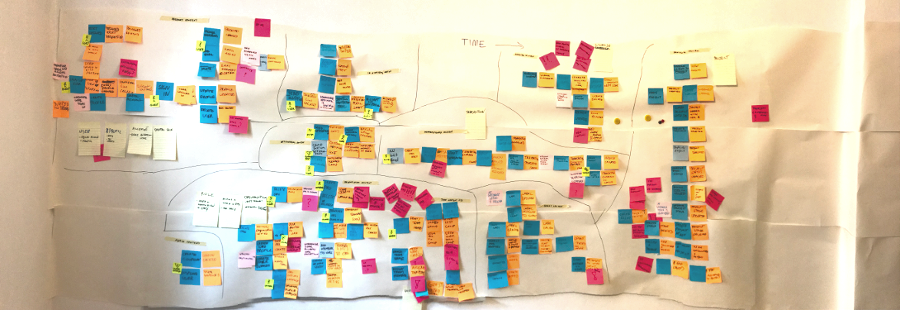
\includegraphics[width=0.75\textwidth]{images/2.1/event-storming}
    \caption{Event Storming Board}
    \label{fig:rlBoard}
\end{figure}

Nachdem initial Domain Events beim \ac{ES} erstellt wurden, soll jedem ein Command vorausgesetzt werden.
Ein Command fungiert hierbei als die Aktion, welche das Event ausgelöst hat.
Dies können Aktionen eines Nutzers oder externen Systems sein.
Während eines Workshops können sogenannte \textit{Hotspots} in Gesprächen entdeckt werden.
Dabei kann es sich um Probleme aber auch Fragen bezüglich des Ablaufs handeln, welche wichtig für die spätere Anwendung werden.

Wie auch das~\ac{DDD} kann Event Storming jederzeit während des Entwicklungsprozesses verwendet werden.
Für die verschiedenen Anwendungsbereiche hat Brandolini mehrere Typen des Event Stormings definiert.
Hierbei bleibt die Methodik an sich die gleiche, allerdings wird das Ziel genauer definiert.\newline
\textbf{Big Picture EventStorming} wird während eines Kick-off Meetings eingesetzt, damit alle Teilnehmer den Inhalt und den Bereich der zur erstellenden Anwendung kennenlernen.
Hierzu ist es nötig, dass alle Interessengruppen vertreten sind, welche innerhalb des Unternehmens existieren und ebenfalls eine Entscheidungsgewalt innehaben.\newline
\textbf{Design Level EventStorming} findet auf einer tieferen Ebene einen Einsatz.
Dabei handelt es sich um das Erstellen möglicher Implementierungen, zum Beispiel, ob Event Sourcing oder andere Techniken aus dem~\ac{DDD} verwendet werden sollen.
Es werden somit Entscheidungen getroffen, welcher in erster Linie die Entwickler betrifft und von diesen am besten zu bewerten ist.\newline
\textbf{Value-Driven EventStorming} bietet einen Einstieg in die Wertstromanalyse (englisch: value-stream mapping).
Anhand einer solchen Analyse ist es möglich den Erhalt von Informationen und der Verarbeitung dieser darzustellen und Probleme zu erkennen.\newline
\textbf{UX-Driven EventStorming} konzentriert sich auf das Erlebnis eines Nutzers/Kunden bei der Benutzung der Anwendung.
Hierbei wird neben der Nutzerfreundlichkeit auch die fehlerfreie Ausführung abgebildet und überprüft.\newline
\textbf{EventStorming as a Retrospective} konzentriert sich darauf einen Ablauf über Domain Events zu definieren und nach
Erweiterungsmöglichkeiten zu suchen, welche Vorteile für die Anwendung bereitstellen können.\newline
\textbf{EventStorming as a Learning Tool} zeigt auch die weiteren Lernchancen innerhalb eines Unternehmens.
Mittels Event Storming ist es somit auch möglich neue Angestellte möglichst schnell auf den aktuellen Stand zu bringen.
Diese Art von Lernchancen ist ebenfalls im~\textbf{Big Picture EventStorming} enthalten.

\subsection{Erweiterung}\label{subsec:erweiterung}
\todo{Hier das vorherige Kapitel abwarten um alle Änderungen/Erweiterungen besser daran fest zu machen.}
\begin{itemize}
    \item Erweiterungen für Wirtschaft (Pages -> daraus generierte Mockups, abgehen von dem "Wir wollen keinen PC benutzen" des ES)
    \item Ideen für die Lehre (Wird in dieser Arbeit nicht näher beleuchtet, da es für den Beleg der Funktionalität nicht mehr möglich ist dies ausreichend in der Bearbeitungszeit zu machen)
    \item ES -> Ablauf von Schritten -> Albert -> Workflow (Arbeitsablauf) beschreibungen -> Mögliche Idee zum besseren Nahebringen von komplexeren Abläufen in Vorlesungen. (Verbildlichung)
\end{itemize}


\section{Technologien}\label{sec:technologien}
Dieses Kapitel gibt einen Überblick über die verwendeten Technologien in der Umsetzung.
Da die Implementierung aus verschiedenen Komponenten besteht, ist dieses Kapitel in drei weitere Unterkapitel aufgeteilt.
Es wird somit getrennt auf die Java Library~\textit{fulibWorkflows}, das Spring Boot Backend des~\textit{fulibWorkflows Web-Editors}
und das zum Editor dazugehörige Frontend, welches mit Angular umgesetzt wurde, eingegangen.

\subsection{fulibWorkflows}\label{subsec:fulibworkflows}
\textit{fulibWorkflows} ist eine Java Library, welche Arbeitsabläufe, im Folgenden "workflows", in \ac{YAML}-Syntax notiert, als Eingabe erhält und daraus
sowohl ein Event Storming Board, im Workflow beschriebene Mockups und Objekt-/ Klassendiagramme generiert.
Welche Form die YAML-Eingabe haben muss und wie die Dateien aussehen und generiert werden, wird in Kapitel~\ref{subsec:workflow-format} erläutert.

\subsubsection{Antlr}\label{subsubsec:antlr}
\ac{Antlr} bietet die Möglichkeit einen Parser über eine eigens geschriebene Grammatik zu generieren.
Die Grammatik muss Links ableitend sein und ist in~\ac{EBNF} definiert.
Der generierte Parser ermöglicht zudem das Aufbauen und Ablaufen eines~\textit{Parse trees}.
Hierdurch ergibt sich die Möglichkeit, während dem Parsen weitere Aktionen durchzuführen, welche den späteren Programmablauf eines Tools unterstützen können.

\begin{listing}[!ht]
    \inputminted{antlr-java}{listings/2.2.1/AntlrExample.g4}
    \caption{Beispiel einer einfachen Grammatik in Antlr}
    \label{listing:grammar-example}
\end{listing}

In Listing~\ref{listing:grammar-example} ist ein Beispiel für eine einfache Grammatik zur Erkennung von mathematischen Gleichungen dargestellt.\cite{antlrOrg}
Hierbei ist es lediglich möglich Zahlen mittels Klammern, Addition, Subtraktion, Multiplikation und Division miteinander zu kombinieren.
Die Länge eines Ausdruckes ist durch den rekursiven Aufbau der Grammatik nicht begrenzt.

\begin{listing}[!ht]
    \begin{minted}{text}
    ((199+2324)*43)/55

    \end{minted}
    \caption{Einfacher mathematischer Ausdruck}
    \label{listing:mathematical-input}
\end{listing}

Die zuvor beschriebene Grammatik kann mittels weiterer Tools auf eine Eingabe geprüft werden.
Eine zulässige Eingabe für die festgelegte Grammatik aus Listing~\ref{listing:grammar-example} ist in Listing~\ref{listing:mathematical-input} dargestellt.
Die Überprüfung auf die Richtigkeit einer Eingabe oder auch der Grammatik kann über Tools bereits vor einer Generierung von Code durchgeführt werden.
Hierzu wurde das Diagramm aus Abbildung~\ref{fig:parse-example} mittels dem Antlr Plugin für IntelliJ generiert.

\begin{figure}[h]
    \centering
    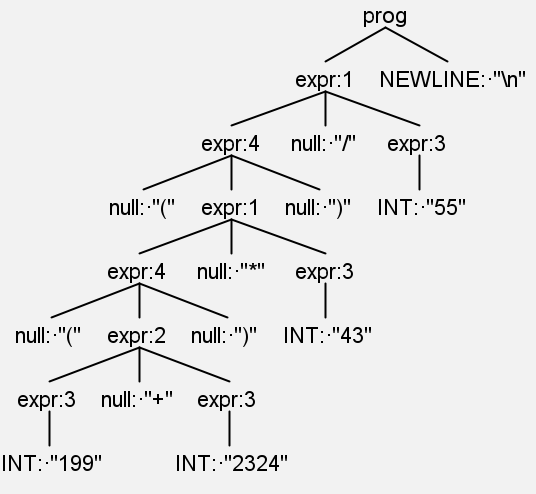
\includegraphics[width=0.3\textwidth]{images/2.2/parseTreeExample}
    \caption{ParseTree für einen mathematischen Ausdruck}
    \label{fig:parse-example}
\end{figure}

Hierbei ist ersichtlich, dass die Wurzel bei der obersten Regel~\textbf{prog} beginnt und alle weiteren Kindknoten durch verschachtelte~\textbf{expr} Regeln kreiert wurden.
Der oberste Teilausdruck ist die Division aus einem komplexeren linken Ausdruck und dem rechten Ausdruck, welcher direkt einer Nummer zugeordnet werden konnte und somit keine weiteren Kindknoten mehr haben kann.
Dies entsteht durch die Unterscheidung bei der Grammatik in Terminale und Nicht-Terminale.
Hierbei werden wie in Listing~\ref{listing:grammar-example} dargestellt Nicht-Terminale Regeln kleingeschrieben und Terminale Regeln werden in Großbuchstaben verfasst.
In der vereinfachten Grammatik sind lediglich ganze Zahlen als Eingabe erlaubt.

Dies sind lediglich die Grundlagen von Antlr, auf die genauere Verwendung des generierten Parsers und Besonderheiten der Grammatik wird in Kapitel~\ref{subsec:antlr-grammatik},
anhand der Implementierung, eingegangen.

\subsubsection{String Template}
\ac{ST} gehört, wie das vorherige \ac{Antlr}, zum~\textit{Antlr Project}.
\ac{Antlr} verwendet ebenfalls \ac{ST}s zur Generierung von formatiertem Text, im Folgenden als \textit{Code} bezeichnet.
Templates (übersetzt: Schablone) ermöglichen es zum Beispiel die feste Syntax einer Programmiersprache mit variablen Werten für
Variablen, Klassen und Methoden zu belegen.
Somit können die generellen Bausteine einer Sprache beliebig gefüllt werden.
Durch diese Funktionalität bieten sich \ac{ST}s sehr gut zur Generierung von Dateien an.
Ursprünglich ist \textit{StringTemplate} eine Java Library, jedoch wurden bereits Portierungen für C\#, Objective-C, JavaScript und Scala erstellt.

Die folgenden Erläuterungen beziehen sich auf die Java Library von \textit{StringTemplate}, da diese in dieser Arbeit verwendet wird.
Die einfachste Möglichkeit für die Verwendung eines String Templates ist in Listing~\ref{listing:simpleTemplate} zu sehen.

\begin{listing}[!ht]
    \inputminted{java}{listings/2.2.1/JavaStringTemplateExample.java}
    \caption{``Hello World!'' - Beispiel mittels StringTemplate}
    \label{listing:simpleTemplate}
\end{listing}

Die Klasse \textit{ST} aus Zeile 3 kann mit einem String initialisiert werden.
In diesem Beispiel wurden als Begrenzer für das zu ersetzende Stück des Textes \textit{<>} verwendet.
Im Anschluss wird dem neuen \textit{ST} Objekt mithilfe der add()-Methode ein bestimmter Wert hinzugefügt.
Der erste Parameter der Methode ist der Bezeichner innerhalb eines Templates, zu beachten ist die Angabe des Bezeichners ohne die Begrenzer.
Der Wert wird als zweiter Parameter übergeben und besitzt in diesem Beispiel den Text \textbf{World}.
Um nun den fertig ersetzten Text aus dem Template und dem übergebenem Wert zu bekommen, muss auf dem \textit{ST} Objekt die Methode render() aufgerufen werden.
Hierbei werden die Platzhalter des Templates durch den zuvor übergebenen Wert ersetzt und als String zurückgegeben.
In Zeile 6 wird nun abschließend der fertige Text auf der Konsole ausgegeben, \texttt{Hello, World!}.
Dieses Beispiel entstammt der offiziellen Webseite von \textit{StringTemplate}.\cite*{stOrg}

Für ein strukturiertes Arbeiten mit vielen Templates bietet \textit{StringTemplate} die Möglichkeit \ac{STG}s zu erstellen.
Hierbei können mehrere Templates in einer Datei beschrieben werden, um aufeinander aufbauende Templates nicht im Code, sondern einer gesonderten Datei zu organisieren.
In diesen Dateien, welche die Dateiendung \textbf{.stg} tragen, können die Begrenzer (eng.: Delimiters) frei gewählt werden.
Dies ist je nach Kontext des Templates nötig, da zum Beispiel die Generierung von HTML-Dateien, welche \textit{<>} als Zeichen zum Abgrenzen von Bereichen verwenden.
Bei der Wahl der Begrenzer sollte somit stets auf die Wahl der Zeichen im Kontext der zu generierenden Sprache geachtet werden.
Zum Parsen einer \ac{STG} wird ein mit Antlr generierter Parser verwendet.\cite*{stgParser}

\begin{listing}[ht]
    \inputminted{c}{listings/2.2.1/Example.stg}
    \caption{Beispiel einer .stg-Datei}
    \label{listing:stgFile}
\end{listing}

Wie zuvor beschrieben ist in Listing~\ref{listing:stgFile} zu erkennen, dass in Zeile 1 die Begrenzer auf~\texttt{\{\}} gesetzt wurden.
Dies hat den Hintergrund, dass in diesem Beispiel ein Text in eine HTML-Datei generiert werden soll.
Hierfür könnten auch die Standardbegrenzer verwendet werden, allerdings müssten dann für Schlüsselwörter wie~\texttt{<span>} die Zeichen < und > mit einem führenden Backslash definiert werden.
Da dies für HTML-Dateien allerdings einen immensen Aufwand bedeutet, macht die Nutzung anderer Begrenzer Sinn.
In Zeile 3 werden für ein~\ac{ST}, sowohl der Name des Templates, als auch Übergabeparameter definiert.
Ein~\ac{ST} wird durch \textit{>>} geschlossen.
Die Begrenzer in Zeile 5 zeigen, dass alles, was sich zwischen Ihnen befindet, einen Übergabeparameter in sich trägt.
Somit ist das Wiederverwenden des Templates und die variable Befüllung gewährleistet.

Um diese Templates nun in einem Java Programm zu verwenden, benötigt es unter anderem die zuvor beschriebenen ST Klasse, sowie
die Klasse \textit{STGroupFile}, welche für die Verwaltung der stg-Datei, als auch deren Templates, benötigt wird.
In Zeile 6 von Listing~\ref{listing:stgJavaFile} ist zu erkennen, dass einem STGroupFile-Objekt bei der Initialisierung eine URL übergeben werden muss.
Diese URL verweist auf die stg-Datei.
Im Anschluss kann, wie in Zeile 8 ersichtlich, über die getInstanceOf()-Methode auf ein bestimmtes Template in der stg-Datei zugegriffen werden.
Hierbei ist es wichtig, keine Fehler bei der Benennung zu machen.
Schließlich ist die weiterführende Verwendung bereits zuvor mittels der ST-Klasse beschrieben worden.

\begin{listing}[!ht]
    \inputminted{java}{listings/2.2.1/JavaSTGExample.java}
    \caption{Nutzung einer STG-Datei in Java}
    \label{listing:stgJavaFile}
\end{listing}

Bei der Ausführung dieses Beispiels wird auf der Konsole der Text aus Listing~\ref{listing:outputSTG} angezeigt.

\begin{listing}[!ht]
    \begin{minted}{html}
<span>
    This test about the university is written in english.
</span>
    \end{minted}
    \caption{STG Ausgabe auf Konsole}
    \label{listing:outputSTG}
\end{listing}

\subsubsection{JSON-Schema}\label{subsubsec:json-schema}
JSON-Schemas sind Schemata, welche den Inhalt einer JSON-/YAML-Datei begrenzen können.
Hierdurch ist es möglich, den Nutzer in seinen Eingaben zu begrenzen und bereits während dem Schreiben einer Datei dabei zu unterstützen sinnvolle Eingaben zu erstellen.
In dieser Arbeit wird lediglich auf die Nutzung der Schema Version 7, die neuste Version, eingegangen, da diese in der Anwendung verwendet wird.

JSON Schemas können Objektstrukturen in beliebiger Tiefe schachteln.
Im folgenden Abschnitt werden die grundlegenden Elemente eines JSON Schemas erläutert.
Weiterführende Funktionalitäten werden anhand der Implementierung in Kapitel~\ref{subsec:schema} näher beleuchtet.

Ein einzelnes Objekt kann zur Verbesserung der späteren Nutzung mit einem Titel und einer kurzen Beschreibung versehen werden.
Diese sind in Listing~\ref{listing:objectSchema} in Zeile 2 und 3 dargestellt.
\textit{title} und \textit{description} dienen lediglich der verbesserten Lesbarkeit für den Entwickler.

\begin{listing}[!ht]
    \inputminted{json}{listings/2.2.1/object.schema.json}
    \caption{Objekt Beispiel eines JSON Schemas}
    \label{listing:objectSchema}
\end{listing}

Einem Element muss stets ein \textit{type}, also ein Typ, zugeordnet werden.
Dies kann entweder ein Objekt, Zeile 4 in Listing~\ref{listing:objectSchema}, oder eine Liste sein.
Einem Objekt können nun \textit{properties} hinzugefügt werden.
Diese besitzen neben einem eindeutigen Bezeichner ebenfalls eine Beschreibung und einen Typen.
Auf dieser Ebene kann der Typ eine Nummer, \textit{integer} in Zeile 8, oder auch ein Text, welches den Typ \textit{string} bekommen würde, sein.
Ist eine der \textit{Properties} ein notwendiges Feld, kann dies mittels des Schlüsselwortes \textit{required} realisiert werden.
Hierbei wird eine Liste an Bezeichnern hinterlegt, welche dem Objekt bereits zugeordnet wurden und somit stets vorhanden sein müssen.
Das Beispiel stammt von der offiziellen JSON Schema Webseite.\cite*{schemaExample}
Sollten einem Objekt keine weiteren properties hinzugefügt werden dürfen, ist dies mit dem Ausdruck aus Listing~\ref{listing:additionalProperties} möglich.

\begin{listing}[!ht]
    \begin{minted}{json}
"additionalProperties": false
    \end{minted}
    \caption{Begrenzung der Properties eines Schemas}
    \label{listing:additionalProperties}
\end{listing}

Wie zuvor bereits beschrieben, kann ein Element auch als Liste deklariert werden.
Dies ist an einem kleinen Beispiel in Listing~\ref{listing:listSchema} dargestellt.
Hierbei ist es möglich die \textit{items} einer Liste genauer zu definieren.
In diesem Beispiel müssen die Elemente einer Liste dem Schema aus dem Beispiel aus Listing~\ref{listing:objectSchema} entsprechen.

Eine JSON-/YAML-Datei, welchem dieses Schema zugrunde liegt, besteht somit aus einer Liste an Produkten.
Durch die Verwendung des \textit{oneOf} Operators in Zeile 6, werden nur Elemente mit dem darunterliegenden Schema akzeptiert.
Bei mehreren Einträgen in der \textit{items} Aufzählung muss immer eines dieser Elemente auf das Objekt in der JSON-/YAML-Datei zutreffen.

\begin{listing}[!ht]
    \inputminted{json}{listings/2.2.1/list.schema.json}
    \caption{Listen Beispiel eines JSON Schemas}
    \label{listing:listSchema}
\end{listing}

Durch ein fest definiertes Schema ist es vielen IDEs, darunter auch IntelliJ und VSCode,
möglich den Entwickler durch Fehlerhervorhebung und Autovervollständigung zu unterstützen.
Hierfür ist es möglich bereits erstellte JSON-Schemas im \textit{SchemaStore} bereitzustellen.
Dies ist eine zentrale Stelle, um JSON-Schemas für IDEs zur Verfügung zu stellen.
Bei dem \textit{SchemaStore} handelt es sich um ein Open-Source-Projekt, bei welchem die Einbringung eines neuen Schemas simpel gestaltet ist.
Es ist möglich ein fertiges Schema fest dort zu hinterlegen, hierdurch muss für jede neue Änderung allerdings ein neuer Betrag erstellt werden.
Dieser bedarf einer Zustimmung einem der Verwalter des \textit{Schema Stores}.
Da dies stets mit einer Verzögerung passiert, ist es möglich eine Verlinkung zu einem Schema zu erstellen.
Somit können Änderungen an einem Schema durchgeführt werden, um diese Änderungen nach dem Hochladen direkt zur Verfügung stellen zu können.
Zum aktuellen Zeitpunkt existieren 439 Schemas, welche durch \textit{SchemaStore.org} für diverse IDEs bereitgestellt werden.\cite*{schemaStore}
Eine Liste aller IDEs, welche diesen Support mittels \textit{schemastore} unterstützen sind unter folgendem
Link zu finden: \url{https://www.schemastore.org/json/#editors}

\subsubsection{fulibTools}
FulibTools ist Teil der Fujaba Tool Suite, auch das in dieser Arbeit erstellte fulibWorkflows ist ein Teil der Fujaba Tool Suite.
Fulib bildet die Grundlage für fulibTools, wobei fulibTools erweiterte Möglichkeiten für die Nutzung von fulib bereitstellt.
Fulib ist ein Codegenerator, welcher mittels einer~\ac{DSL}, Modelle als Diagramme darstellen kann.\cite*{fulib}
Dies begrenzt sich nicht nur auf Klassenmodelle, sondern ist auch für Objektmodelle einsetzbar.
FulibTools ist eine Erweiterung, da die Generierung der Diagramme auch abseits der eben erwähnten DSL funktioniert.\cite*{fulibTools}
Hierdurch bietet sich die Möglichkeit Objektmodelle über ein spezielles YAML-Format oder ein Java Objektmodell zur Laufzeit zu generieren.
Gleiches gilt für Klassenmodelle.
Die Verwendung von FulibTools ist somit für diese Arbeit eine bessere Wahl, als \textit{Graphviz}, eine Bibliothek zur Generierung von Diagrammen, direkt zu verwenden.
Dies ist der Fall, da FulibTools bereits die Arbeit der Verarbeitung einer Eingabe übernimmt und hierdurch leichter für ein weiteres Tool der Fujaba Tool Suite zu verwenden ist.


\subsection{Frontend des Web-Editors}\label{subsec:fulibworkflows-web-editor}
Der Web-Editor für fulibWorkflows besteht aus einem Frontend und einem Backend.
Dieses Kapitel beschäftigt sich mit den Technologien, welche für das Frontend verwendet werden.
Hierbei wurde die Entscheidung über die verwendeten Technologien für die Integration des Editors in die Webseite \url{fulib.org} getroffen.
Auf diese Integration wird in Kapitel~\ref{ch:fazit} näher eingegangen.

\subsubsection{Angular}
Die Grundlage für das Frontend ist Angular.
Angular ist ein Framework für das Designen von Applikationen und gleichzeitig eine Entwicklungsplattform\cite*{angular}.
Für Entwickler ist das Angular Command-Line-Interface ein wichtiger Bestandteil bei der Entwicklung mit Angular.
Neben der Generierung einer neuen Anwendung können ebenfalls neue Komponenten, Services und Module generiert werden.
Die \textit{Komponenten} dienen der Strukturierung einer Anwendung und enthalten verschiedene Abschnitte ebendieser.
Hierbei besteht ein großer Vorteil darin, Komponenten modular zu gestalten.
Dies bedeutet, dass Komponenten so entwickelt werden, dass diese in der Anwendung wiederverwendet werden können, sollte dies möglich sein.
Eine Komponente besteht aus drei einzelnen Bereichen:

\begin{enumerate}
    \item Der Logik, welche in Typescript verfasst wird.
    \item Einem Template, welches eine HTML-Datei ist.
    \item Styles, welche im Template eingebunden werden können, um die Oberfläche grafisch zu verändern.
\end{enumerate}

Im Template werden neben den Styles auch Bestandteile des Code-Segments verwendet, um Daten dynamisch anzeigen zu können.
Ein neu generiertes Angular Projekt bietet allerdings nur die Grundlage einer Anwendung.
Um weitere Funktionalitäten in der Anwendung verwenden zu können, können sogenannte Package Manager wie \textit{npm} oder \textit{yarn}
verwendet werden, um neue Bibliotheken einzubinden.

Auf weitere Erklärungen wird an dieser Stelle verzichtet, da Angular in Gänze zu erklären den Rahmen dieser Arbeit überschreiten würde.
In Kapitel~\ref{sec:editor-frontend} wird auf weitere Funktionen genauer eingegangen und diese anhand der Implementierung erklärt.
Folgend werden Bibliotheken erläutert, welche die wichtigsten Bestandteile der Anwendung ermöglichen.

\subsubsection{Bootstrap}
Um eine Oberfläche zu gestalten, welche einheitlich mit der von \textit{fulib.org} sein soll, wurde Bootstrap zum
Stylen der Oberflächenelemente verwendet.
Bootstrap bietet diverse Komponenten wie Eingabefelder, Buttons, Menüs, Pop-Ups und viele weitere.
Neben den Styles enthalten diese auch zusätzliche Funktionen, welche im Kontext der Komponente sinnvoll sind.
Dabei bleibt es weiterhin abänderbar, um dem Entwickler mehr Freiheiten zur Gestaltung einer Oberfläche zu geben.
Weiterhin ermöglicht es Bootstrap das Layout, also die Anordnung, von Komponenten auf einer Seite festzulegen.
Dies beginnt bei der Größe einer Komponente bis hin zu der Anordnung in der Horizontalen und Vertikalen\cite*{bs}.

Zusätzlich zu Bootstrap wurden Bootstrap Icons verwendet, um die Oberfläche mit Symbolen zu versehen.
Hierbei handelt es sich um eine Sammlung von rund über 1500 Icons, welche frei verwendbar sind\cite*{bsIcons}.

\subsubsection{CodeMirror}
CodeMirror ist ein Texteditor, welcher in JavaScript geschrieben wurde und somit in Web-Anwendungen verwendet werden kann.
Es gibt zahlreiche Optionen, um CodeMirror an die Bedingungen der zu bauenden Anwendung anzupassen.
Neben zahlreichen Programmiersprachen, welche durch das Hervorheben von Schlüsselwörtern und der Überprüfung der Syntax emuliert werden können,
ist es möglich CodeMirror zu einer eigenen, individualisierten IDE zu konfigurieren.
Erweiterungen für einen CodeMirror sind die sogenannten Add-Ons.
Hierbei gibt es neben vielen bereits vorhandenen Erweiterungen auch die Möglichkeit eigene Add-Ons zu erstellen.
Hierzu zählt unter anderem das zuvor erwähnte farbliche Hervorheben von Schlüsselwörtern, auch Highlighting genannt, wie auch die
Überprüfung des Codes auf die Syntax der eingestellten Programmiersprache\cite*{cm}.

Für eine einfache Einbindung in ein Angular-Projekt existieren bereits mehrere Bibliotheken, welche eine CodeMirror-Komponente bereitstellen.
Bei dieser Komponente können nicht nur Optionen übergeben, sondern auch der Inhalt eines CodeMirrors, also den geschriebenen Code, aus der Komponente
extrahiert werden.
In dieser Arbeit wird hierzu ngx-codemirror von Scott Cooper verwendet\cite*{ngxcm}.


\subsection{fulibWorkflows Web-Editor Backend}\label{subsec:backend}
Das folgende Kapitel beschäftigt sich mit dem zweiten Bestandteil des Web-Editors, das Backend.
Vom Frontend wird eine YAML-Beschreibung ans Backend geschickt, in diesem wird dies als Eingabe für fulibWorkflows verwendet.
Da fulibWorkflows eine Java-Bibliothek ist, benötigt es ein Backend, welches auf Java basiert.

\subsubsection{Spring Boot}
Mittels \textit{Spring Boot} ist es möglich schnell und ohne zusätzliche Konfiguration eine auf \textit{Spring} basierende Applikation zu erstellen.\cite*{springBoot}
Spring ist ein Framework, welches sich als Ziel gesetzt hat Java Programmierung zu vereinfachen und zu verschnellern, allerdings keine Einbußen
bei Geschwindigkeit, Komplexität und Produktivität zu machen.\cite*{spring}
In diesem Kapitel wird sich mit der Erstellung eines Rest-Services befasst.
Ein Rest-Service stellt Endpunkte bereit, welche über REST angesprochen werden können.
Diese eignen sich zur Nutzung als simples Backend.

\begin{figure}[h]
    \centering
    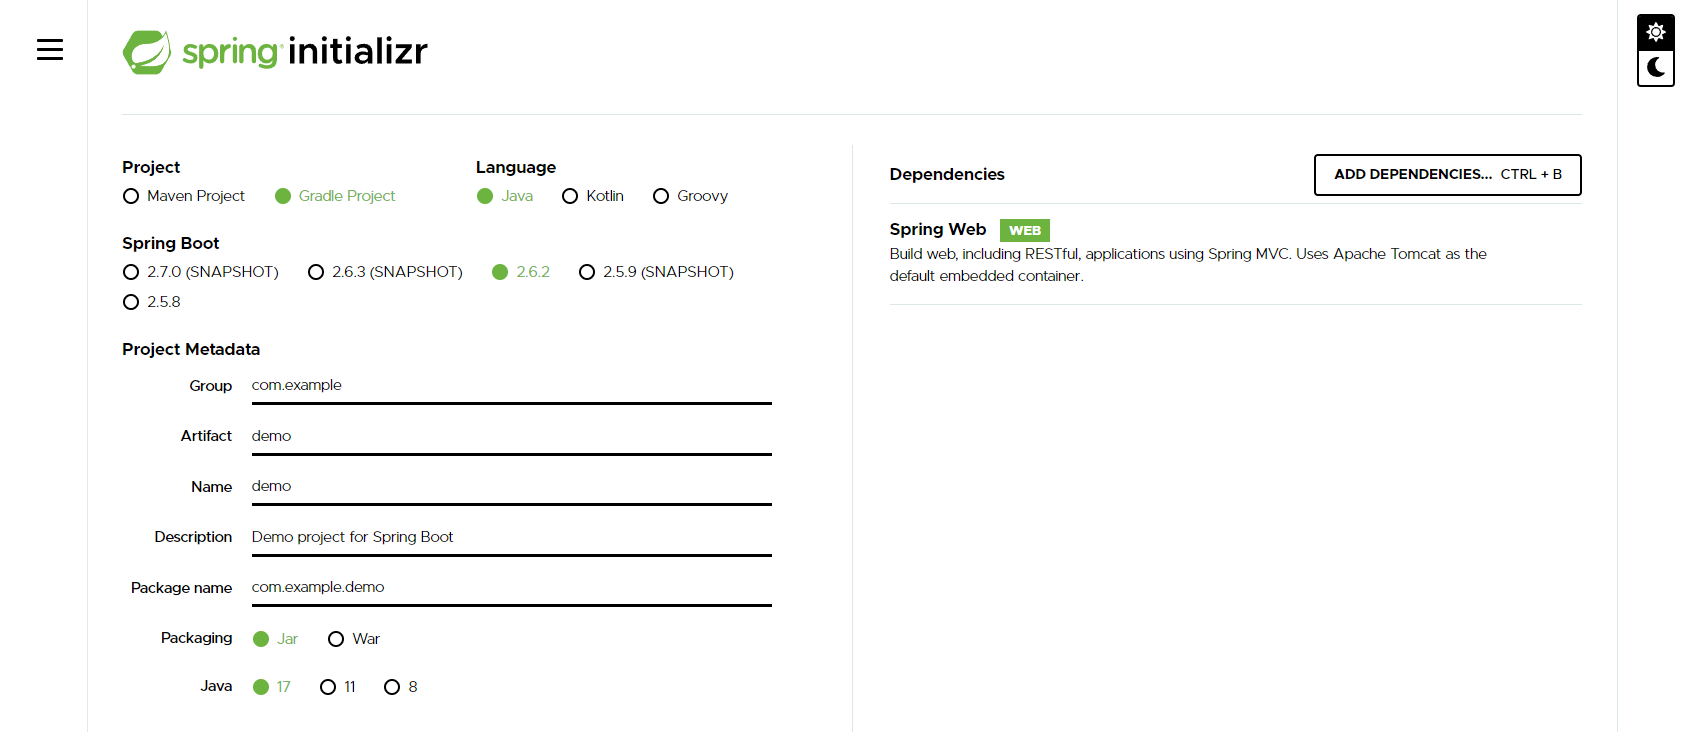
\includegraphics[width=1.0\textwidth]{images/2.2/spring-init}
    \caption{Spring Initalizr für eine Web Anwendung}
    \label{fig:spring-init}
\end{figure}


Das Anlegen eines Spring Boot Projektes kann durch den \textit{Spring Initializr} erledigt werden.\cite*{sbinit}
In Abbildung~\ref{fig:spring-init} ist dieser zu sehen.
Hierbei können diverse Einstellungen getätigt werden, um das zu generierende Projekt an die Anforderungen des Generierenden anzupassen.
Die Abbildung zeigt die getätigten Einstellungen, um ein Gradle Projekt mit Java, Version 17, als Programmiersprache zu generieren.
Ebenfalls kann die Version von Spring Boot eingestellt werden.
Zusätzliche Dependencies können im rechten Bereich des \textit{Spring Initializrs} hinzugefügt werden.
In diesem Fall wurde \textbf{Spring Web} ausgewählt, wodurch die wichtigsten Dependencies für eine REST Applikation bereits enthalten sind.

Das aus den vorherigen Einstellungen beschriebene Projekt ist bereits ein fertiges Backend, welches direkt ausgeführt werden kann.
Durch sogenannte Annotations, welche mit einem @ gekennzeichnet werden, ist es möglich weitere Endpunkte für das Backend zu definieren.
Auf die genaueren Funktionen, welche mittels Annotations implementiert werden können, wird in Kapitel~\ref{sec:editor-backend} eingegangen, anhand von Beispielen der Implementierung.



\subsection{Deployment}\label{subsec:deployment}
\todo{this}
Ein Web Editor will natürlich für alle erreichbar sein.
Und fulibWorkflows muss auch irgendwo bereitgestellt werden, damit es das Backend und alle anderen
interessierten benutzen können.

\subsubsection{MavenCentral}\label{subsubsec:mavencentral}
\todo{this}
MavenCentral ein wirklicher Hussarones was das publishen angeht.
Glücklicherweise ist fulibWorkflows Teil der Fujaba Tool Suite, wodurch die benötigten
Zugriffsrechte bereits vorhanden und andere Libraries bereits gepublished wurden.
Hierdurch war es recht schnell möglich mit dem zuvor erworbenem Wissen fulibWorkflows
zu publishen.

\subsubsection{Heroku}\label{subsubsec:heroku}
\todo{this}
Der Web-Editor soll immer erreichbar sein.
Dies ist durch Heroku nur bedingt möglich.
Heroku bietet allerlei Möglichkeiten verschiedenste Anwendungen bereitzustellen.
Auch mit einem kostenlosen Plan ist es ohne Probleme möglich solch kleine Anwendungen bereitzustellen.

FE Deployment war easy, auch wenn ich erstmal wieder in eins meiner früheren Projekte gucken musste.
BE Deployment war kniffliger, doch man ist nie der erste der eine Spring Boot application
auf Heroku deployen will.
Daher Tutorial reingefahren und ab ging der gebutterte Lachs.



\chapter{Implementierung}\label{ch:implementierung}
Dieses Kapitel erläutert die Implementierung der in dieser Arbeit erstellten Anwendungen.
Diese wird anhand der im vorherigen Kapitel erläuterten Technologien genauer erklärt.
Hierbei beschäftigt sich Kapitel~\ref{sec:fulibworkflows2} mit fulibWorkflows, Kapitel~\ref{sec:editor-frontend} mit dem Frontend des
fulibWorkflows Web-Editors und abschließend Kapitel~\ref{sec:editor-backend} mit dem dazugehörigen Backend.

\section{fulibWorkflows}\label{sec:fulibworkflows2}
Bei~\textit{fulibWorkflows} handelt es sich um eine Java-Bibliothek, welche Workflow-Beschreibungen als Eingabe erhält, diese Eingabe
parst und daraus HTML-/FXML-Mockups, Objektdiagramme und Klassendiagramme generiert.
Das Parsen wird über einen von \ac{Antlr} generierten Parser übernommen, hierzu wird in Kapitel~\ref{subsec:antlr-grammatik} genauer auf
die zugrundeliegende Grammatik eingegangen.
Zudem wird auf die Limitationen des Parsers und der generierten Mockups eingegangen.

\subsection{Workflow-Format}\label{subsec:workflow-format}
Bevor in Kapitel~\ref{subsec:datenmodell} auf den Parser und das Datenmodell einer Workflow-Beschreibung eingegangen wird,
ist es nötig das Format in welcher ein Workflow beschrieben werden muss, näher zu beleuchten.
Die Grundlage des Formats bildet~\ac{YAML}.
Wobei das Format durch ein JSON-Schema stark begrenzt ist.
Näheres zu den Beschränkungen der Syntax wird in Kapitel~\ref{subsec:schema} erklärt.

\begin{listing}[!ht]
    \inputminted{yaml}{listings/3.1.1/allNotes.es.yaml}
    \caption{Beispiel aller vorhandenen Post-its\textsuperscript{\textregistered}}
    \label{listing:workflowNotes}
\end{listing}

In Listing~\ref{listing:workflowNotes} sind alle möglichen Post-its\textsuperscript{\textregistered} aufgelistet.
Im weiteren Verlauf wird für einen Post-it\textsuperscript{\textregistered} das Wort Zettel verwendet, da es sich bei jedem Element in der Beschreibung um einen einzelnen Zettel aus dem Event Storming handelt.
Als Beispiel für einen Workflow ist hierbei die Registrierung eines neuen Benutzenden auf einer Webseite in vereinfachter Form dargestellt.
Folgend werden alle verwendbaren Zettel aus der aktuellen Version, v0.4.0, von fulibWorkflows aufgelistet und deren Funktion erläutert.

\largerText{workflow}

Zum Darstellen eines oder mehrerer Workflows benötigt es den \textit{workflow}-Zettel.
Diesem kann nur ein Name zugeordnet werden, allerdings werden alle weiteren Zettel unter einem workflow-Zettel ebendiesem Workflow zugewiesen.
Pro Workflow-Beschreibung benötigt es somit mindestens einen workflow-Zettel.
Im vorherigen Beispiel gibt es einen Workflow mit dem Namen~\textit{User Registration}.

\largerText{service}

Durch den \textit{service}-Zettel werden Services bereitgestellt.
Diese sind einzig zur Strukturierung des Workflows und dem später daraus entstehenden~\ac{ES}-Board da.
Hiermit kann erreicht werden, dass die nach einem service-Zettel folgenden Zettel von dem vorherigen Service ausgeführt werden.
Im Beispiel aus Listing~\ref{listing:workflowNotes} gibt es nur einen Service, dieser kümmert sich um die Nutzerverwaltung, daher
stammt auch der Name~\textit{User management}.

\largerText{problem}

Falls während einem Event Storming an einem bestimmten Punkt innerhalb eines Workflows Fragen bei den Beteiligten aufkommen,
können diese mittels \textit{problem}-Zettel festgehalten werden.
Gleiches gilt für Probleme, welche bisher auftraten, allerdings noch nicht festgehalten wurden.
Somit ist es möglich zusätzliche Informationen, welche nicht zum eigentlichen Workflow gehören, darzustellen und in der
späteren Entwicklung genauer zu betrachten.
Im obigen Workflow Beispiel, gibt es das Problem, dass das Validieren einer E-Mail enorm lange dauert, siehe Zeile 20.

\largerText{event}

Aus dem~\textit{Domain Event} aus dem Event Storming ist die verkürzte Version \textit{event} als Indikator für einen weiteren Zettel geworden.
Hierbei wird eine Beschreibung eines Events in der Vergangenheitsform als Bezeichnung verwendet.
Dies bezieht sich auf eine Aktion, welche innerhalb eines Workflows aufgetreten ist.
Wie in Listing~\ref{listing:workflowNotes} in Zeile 24 und ab Zeile 30 zu sehen, können event-Zettel allein stehen oder mit weiteren Informationen
angereichert werden.
Weitere Informationen, die einem Event zugeordnet sind, repräsentieren Daten, welche zu der ausgeführten Aktion gehören.

\largerText{user}

Ein \textit{user}-Zettel ist sehr ähnlich zu einem \textit{service}-Zettel.
Einem User wird ein Name zugeordnet.
Dieser Zettel dient ebenfalls der Strukturierung eines Workflows und leitet einen Abschnitt ein, welcher aktiv von einem
Nutzenden durchgeführt werden muss.
Im Beispiel-Workflow existiert ein User, welcher den Namen Karli trägt, dies ist in Zeile 3 zu sehen.

\largerText{policy}

Eine \textit{policy} ist wie auch beim \textit{event} eine Abstrahierung eines Begriffes aus dem Event Storming.
Ein \textit{policy}-Zettel beschreibt somit einen Automatismus, welcher aufgrund eines vorherigen Events einen bestimmten
Ablauf an Schritten ausführt.
Im Beispiel aus Listing~\ref{listing:workflowNotes} reagiert die policy aus Zeile 18 auf den vorherigen Command, um automatisch zu prüfen,
ob die eingegebene E-Mail valide ist.

\largerText{command}

Ein \textit{command}-Zettel stellt die Interaktion eines Nutzenden mit einer Webseite oder Applikation dar.
Im Falle des obigen Beispiels wird in Zeile 16 der Klick auf den Knopf \textit{Register} aus der darüber aufgeführten Page simuliert.
Dies ist aus der kurzen Beschreibung des Commands zu entnehmen.

\largerText{externalSystem}

Wie auch bei dem \textit{service} und \textit{user} dient der \textit{externalSystem}-Zettel dazu, einen Workflow zu strukturieren.
In diesem Fall bedeutet dies, dass Aktionen oder Daten von einem System ausgeführt/gesendet werden, welche nicht Teil der zu entwickelnden
Software sind, für welche das aktuelle Event Storming durchgeführt wird.
In Zeile 20 des Beispiels existiert ein externalSystem, welches für die Validierung einer E-Mail-Adresse zuständig ist.
Es kann sich dabei um ein System handeln, welches von einer anderen Firma oder einem separaten Team entwickelt wird.

\largerText{data}

Wie in Kapitel~\ref{sec:event-storming} bereits erwähnt, ist \textit{data} eine Erweiterung des Event Stormings.
Ein \textit{data}-Zettel benötigt als Bezeichner eine besondere Form, diese besteht zuerst aus einer Klassenbezeichnung und anschließend einem Namen für das Objekt.
Dies ist nötig, um im späteren Verlauf das Aufbauen eines Datenmodells zu gewährleisten und ein Klassendiagramm und mehrere Objektdiagramme generieren zu können.
Wie auch bei dem \textit{event}-Zettel kann auch einem \textit{data}-Zettel zusätzliche Informationen übergeben werden.
Auf welche Art und Weise diese aufgebaut sein müssen und welche Funktionen diese innehaben, darauf wird in Kapitel~\ref{subsubsec:objektdiagramme} genauer eingegangen.
In Zeile 35 unseres Beispiels wird ein \textit{User} mit den aus dem Event stammenden Informationen zu Username, E-Mail und Passwort angelegt.

\largerText{page}

Der \textit{page}-Zettel ist ebenfalls eine Erweiterung zum klassischen Event Storming.
Aus den \textit{page}-Zetteln eines Workflows werden später Mockups generiert, wie dies genau funktioniert wird in Kapitel~\ref{subsubsec:mockups-html/fxml} erläutert.
An diesem Punkt ist es wichtig, die Restriktionen einer \textit{page} zu erläutern.
Eine Page besteht aus einer Liste an Elementen, hierbei steht \textit{pageName} für den Bezeichner der Page und wird im Mockup nicht dargestellt.
Um die Oberfläche einer Applikation zu beschreiben, existieren vier Elemente, welche beliebig oft verwendet werden können.

Ein Text-Element enthält einen Text, welcher entweder zur Verwendung als Überschrift, Bezeichner oder Trenner verwendet werden kann.
Um Daten in einer Applikation eingeben zu können, gibt es das \textit{input}- und das \textit{password}-Element.
Bei beiden handelt es sich um Eingabefelder, mit dem Unterschied, dass bei dem \textit{password}-Element der eingetippte Inhalt mit Punkten ersetzt wird.
Der Bezeichner, welcher einem Input oder Password hinterlegt wird, wird als Platzhalter im Eingabefeld und als Label über ebendiesem angezeigt.
Um die Variationen der Mockups zu erweitern und diese mit beispielhaften Eingaben zu füllen, können sowohl dem \textit{input}- als auch \textit{password}-Element
ein Attribut namens \textit{value} zugeordnet werden.
Dabei handelt es sich um den Inhalt des Eingabefeldes, welches im Mockup angezeigt wird.
Zuletzt kann ein Knopf mithilfe eines~\textit{button}-Elements erstellt werden, dabei wird der Bezeichner als Inhalt des Knopfes dargestellt.
Das \textit{button}-Element kann ebenfalls mit einem weiteren Attribut versehen werden.
Mit dem Attribut \textit{targetPage} kann dem Knopf der Name einer Seite übergeben werden, welche innerhalb der workflow-Datei definiert wurde.
Dafür ist es notwendig, dass die erstellten Pages unterschiedliche Namen besitzen.
Dieses Attribut entfaltet seine Funktionalität im Web-Editor zu fulibWorkflows, da es somit möglich ist eine lose Verlinkung zwischen einem Button und einer Page
zu erzeugen.
Näheres zu der Verwendung und der Umsetzung folgt in Kapitel~\ref{subsec:darstellung-generierter-dateien}.

Eine Oberfläche kann nur von oben nach unten beschrieben werden, eine weitere Limitierung ist, dass es nicht möglich ist mehrere Elemente in eine Reihe zu ordnen.
Hierdurch ist das Designen eines Mockups durch die geringe Anzahl an Elementen stark begrenzt und kann lediglich für
simple Benutzeroberflächen verwendet werden.


\subsection{JSON-Schema}\label{subsec:schema}
Wie im vorherigen Kapitel bereits erwähnt bedient sich die Beschreibung eines Workflows grundlegend der Syntax von~\ac{YAML}.
In Kapitel~\ref{subsubsec:json-schema} wurden bereits die Grundlagen für JSON-Schemas geschaffen, in diesem Kapitel wird das erstellte
fulibWorkflows-Schema genauer betrachtet.
Das komplette Schema ist in dem referenzierten fulibWorkflows-Repository im Anhang hinterlegt, da dieses zu lang ist, um es übersichtlich in diesem Kapitel zu erläutern.
Dadurch wird nur auf die wichtigsten Punkte der Implementierung eingegangen.
Um die Lesbarkeit für Entwickelnde zu verbessern, ist das Schema in zwei Dateien aufgeteilt.

\begin{listing}[!ht]
    \inputminted{json}{listings/3.1.2/page.json}
    \caption{Referenzieren eines anderen Schemas}
    \label{listing:schema-split}
\end{listing}

Listing~\ref{listing:schema-split} ist eine minimale Version des eigentlichen Schemas, in welchem dennoch die wichtigsten Funktionen dargestellt sind.
Das fulibWorkflows-Schema enthält die Definitionen und die Festlegung der erlaubten Elemente in der obersten Liste.
Durch das Schema werden nur JSON-/YAML-Dateien akzeptiert, welche aus einer Liste an Elementen bestehen.
Hierbei sind die Elemente jedoch festgelegt, dies ist durch die Spezifikation ab Zeile 19 umgesetzt.
Ein \textit{item} darf nur aus einem der Elemente bestehen, welche in der Auflistung ab Zeile 22 aufgezählt sind.
Um die Lesbarkeit zu vereinfachen und die Schachtelungstiefe möglichst gering zu halten, werden nur die erlaubten Elemente referenziert.
Die referenzierten Elemente wurden im ersten Teil des Schemas, ab Zeile 4, definiert.
Für jedes der im vorherigen Kapitel erwähnten Zettel gibt es ein Element im Schema.
Die Definitionen der Elemente, welche nicht in Listing~\ref{listing:schema-split} dargestellt sind, enthalten Standardwerte, welche bereits in Kapitel~\ref{subsubsec:json-schema} erläutert wurden.
Die Definition der Page ist jedoch ein Sonderfall, welcher durch das Aufteilen in mehrere Dateien entstanden ist.
Es ist möglich weitere Schemas aus einer anderen Datei zu importieren, dies ist in Zeile 11 ersichtlich.
Auch dort gibt es Referenzen, allerdings referenzieren diese nicht auf eine im Schema befindliche Definition, sondern auf die Page-Definition aus der \textit{page.schema.json}-Datei.
Die Aufteilung wurde durchgeführt, da die Page eine Liste ist und ebenfalls fünf eigene Elemente definiert.
Allein das Page-Schema beläuft sich auf 93 Zeilen und umfasst somit allein die Hälfte des Parent-Schemas.

Wie in Kapitel~\ref{subsubsec:json-schema} bereits erwähnt, ist das fulibWorkflows-Schema ebenfalls bei Schemastore.org hinterlegt.
Das Schema wird automatisch auf Dateien mit der Dateiendung \textit{.es.yaml} vom Editor angewendet.
Dadurch ist es zum Beispiel in IntelliJ möglich Autovervollständigung für fulibWorkflows zu bekommen und auf Fehler hingewiesen zu werden.

\begin{figure}%
    \centering
    \subfloat[\centering Leere Datei]{{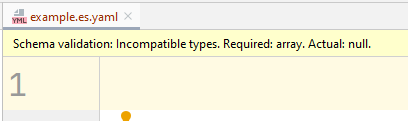
\includegraphics[width=6cm]{images/3.1/Empty} }}%
    \qquad
    \subfloat[\centering Fehlerhafte Eingabe]{{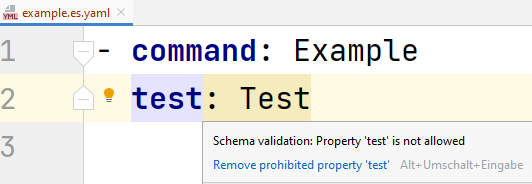
\includegraphics[width=7cm]{images/3.1/fails} }}%
    \caption{Fehleranzeige in IntelliJ}%
    \label{fig:errors-schema}%
\end{figure}

In Abbildung~\ref{fig:errors-schema} ist das Hervorheben von Fehlern in IntelliJ dargestellt, welches durch das JSON-Schema generiert wird.
In Abbildung~\ref{fig:errors-schema}((a)) ist die Datei leer, wodurch die Schema Validierung anschlägt und den Entwickelnden darauf hinweist, dass ein Array, also eine Liste an Elementen, benötigt wird.
Sobald ein Element begonnen wird, wird diese Warnung nicht mehr angezeigt.
Sollte der Entwickelnde wiederum ein Element hinzufügen, welches keinem der definierten Elemente des Schemas entspricht, wird die Meldung aus Abbildung~\ref{fig:errors-schema}((b)) angezeigt.
Da ein Command keine zusätzlichen Attribute/Properties akzeptiert, dennoch eines hinzugefügt wurde, besagt der Fehler, dass es nicht erlaubt ist weitere Attribute hinzuzufügen.

\begin{figure}%
    \centering
    \subfloat[\centering Alle Elemente]{{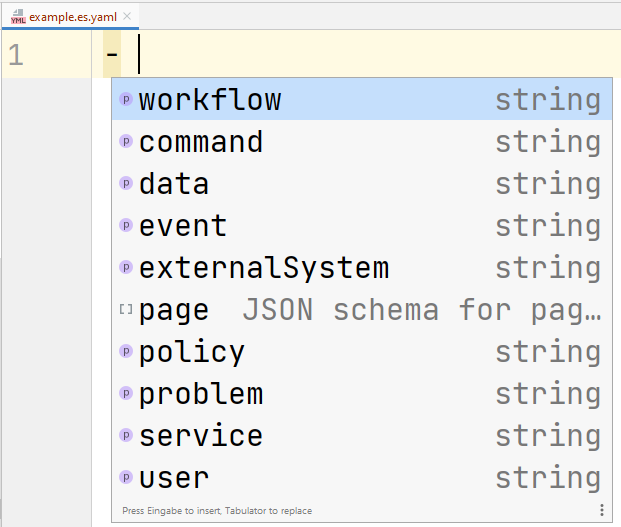
\includegraphics[width=6cm]{images/3.1/all} }}%
    \qquad
    \subfloat[\centering Page Elemente]{{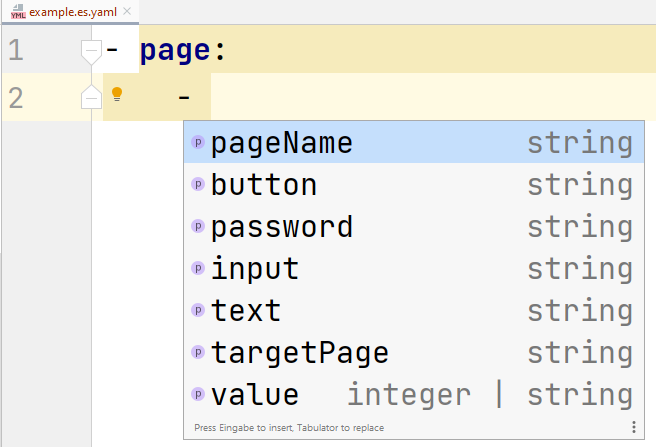
\includegraphics[width=6cm]{images/3.1/page} }}%
    \caption{Autovervollständigung in IntelliJ}%
    \label{fig:completion-schema}%
\end{figure}

Wie zuvor erwähnt ermöglicht ein Schema jedoch nicht nur das Hervorheben von Fehlern, sondern unterstützt den Entwickelnden zusätzlich durch Autovervollständigung.
Dies ist in Abbildung~\ref{fig:completion-schema} dargestellt.
Hierbei werden aufgrund des Kontextes verschiedene Möglichkeiten von zu erstellenden Elementen vorgeschlagen.
Auf oberster Ebene werden alle erlaubten Schlüsselwörter für Elemente angezeigt, dies ist in Abbildung~\ref{fig:completion-schema}((a)) dargestellt.
Hierbei fällt auf, dass die Elemente für eine Page nicht angezeigt werden, dies ist jedoch der Fall, sobald der Kontext dies zulässt.
Während der Entwickelnde ein page-Element definiert, werden wie in Abbildung~\ref{fig:completion-schema}((b)) dargestellt die Schlüsselwörter für Page-Elemente vorgeschlagen.


\subsection{Antlr-Grammatik}\label{subsec:antlr-grammatik}
Da die möglichen Eingaben durch das zuvor beschriebene JSON-Schema bereits verringert wurden, fiel die Wahl der Verarbeitung der YAML-Eingabe auf einen durch Antlr generierten Parser.
Dieser bietet die Möglichkeit, während dem Parsen weitere Aktionen durchzuführen und in dem Fall dieser Anwendung ein Datenmodell aus der Eingabe zu erstellen.
Das Datenmodell wird im folgenden weiterverarbeitet und bietet somit eine Grundlage für die Generierung, auf welche im folgenden Kapitel eingegangen wird.

Wie in Kapitel~\ref{subsubsec:antlr} bereits beschrieben, ist die Grundlage eines Antlr-Parsers die dazugehörige Grammatik, welche nun beleuchtet wird.
Die komplette Grammatik ist im referenzierten fulibWorkflows-Repository im Anhang hinterlegt, in diesem Kapitel werden lediglich Ausschnitte daraus verwendet.
Im Folgenden wird anstatt Zettel zur Beschreibung eines Post-its die englische Übersetzung ``Note'' verwendet, um einen direkten Bezug zu den nachfolgenden Listings herzustellen.

\begin{listing}[!ht]
    \inputminted[firstnumber=5]{antlr-java}{listings/3.1.3/Main.g4}
    \caption{Grammatik für Workflows}
    \label{listing:main-grammar}
\end{listing}

Zuerst wird die grundlegende Struktur einer Datei festgelegt, dies ist durch die drei Regeln in Listing~\ref{listing:main-grammar} dargestellt.
Da eine Datei mehrere Workflows beinhalten kann, ist die oberste Regel in Zeile 5 der Startpunkt des Parsers.
Da als Eingabe eine YAML-Datei ist, heißt die oberste Regel \textit{file} und erfordert mindestens einen~\textit{workflow}.
Ein~\textit{workflow} besteht immer aus einem workflow-Note und beliebig vielen event-Notes, wobei diese immer mit einer Leerzeile von einander getrennt sind.
Die Spezifikation ist aufgrund der YAML-Syntax notwendig.
Ein event-Note ist immer einem von drei Typen zuzuordnen, wobei nach einem Note beliebig viele Leerzeilen folgen können.

\begin{listing}[!ht]
    \inputminted[firstnumber=11]{antlr-java}{listings/3.1.3/Note.g4}
    \caption{Grammatik für Notes}
    \label{listing:note-grammar}
\end{listing}

Die Unterscheidung zwischen normal-/extended-Note, workflow und page erfolgt durch das Schlüsselwort, welches zwischen Bindestrich (\textbf{MINUS}) und Doppelpunkt (\textbf{NAME}) befindet.
Sowohl ein workflow-Note als auch die normal-Notes besitzen lediglich nach dem Doppelpunkt einen Wert, welcher durch \textbf{NAME} gekennzeichnet ist.
Dies ist in Listing~\ref{listing:note-grammar} in Zeile 11 und 13 dargestellt.
Ein extended-Note besitzt neben dem Wert zusätzliche Attribute, welche in einer neuen Zeile beschrieben werden.
Die Anzahl der Attribute ist beliebig, es ist somit erlaubt einen extended-Note ohne weitere Attribute anzugeben.
Die Page ist wie zuvor bereits erwähnt ein Sonderfall, welches sich auch in der Grammatik widerspiegelt.
Dem Schlüsselwort \textit{page} folgt ein gesonderter Doppelpunkt und anschließend eine Liste von neuen Elemente.

\begin{listing}[!ht]
    \inputminted[firstnumber=30]{antlr-java}{listings/3.1.3/Keywords.g4}
    \caption{Schlüsselwörter zum Identifizieren von Notes}
    \label{listing:note-ids}
\end{listing}

Die zuvor erwähnten normal-Notes bestehen wie in Listing~\ref{listing:note-ids} Zeile 30 und 31 dargestellt aus \textit{externalSystem}, \textit{service}, \textit{command}, \textit{policy}, \textit{user} und \textit{problem}.
Diese erhalten lediglich einen Bezeichner und erlauben keine weiteren Attribute.
Zu den extended-Notes zählen lediglich \textit{event} und \textit{data}.
Diese erhalten weitere Attribute, um Daten, welche zwischen Services verschickt werden, darstellen zu können.

\begin{listing}[!ht]
    \inputminted[firstnumber=19]{antlr-java}{listings/3.1.3/Attribute.g4}
    \caption{Grammatik von Attributen}
    \label{listing:attributes}
\end{listing}

Attribute werden eingerückt und enthalten neben einem Bezeichner (\textbf{NAME}) einen dazugehörigen Wert (\textit{value}).
Ein Wert kann entweder ein Text, eine Nummer oder eine Liste sein, wobei eine neue Zeile optional ist.
Die dazugehörigen Regeln sind in Zeile 19 und 21 aus Listing~\ref{listing:attributes} vermerkt.

Wie in Listing~\ref{listing:values} zu sehen ist, ist der akzeptierte Text auf eine feste Menge an verschiedenen Zeichen begrenzt.
Ein Text muss stets mit einem Buchstaben beginnen, ungeachtet ob groß- oder kleingeschrieben.
Darauf können Zahlen, Sonderzeichen und weitere Wörter folgen.
Die Sonderzeichen sind in Zeile 36 genauer beschrieben.

\begin{listing}[!ht]
    \inputminted[firstnumber=36]{antlr-java}{listings/3.1.3/Values.g4}
    \caption{Grammatik von Werten}
    \label{listing:values}
\end{listing}

Eine Nummer kann lediglich eine ganze Zahl sein, führende Nullen sind erlaubt.
Die Möglichkeit als Wert eine Liste angeben zu können, basiert auf der Möglichkeit Objekt- und Klassendiagramme mit fulibWorkflows zu generieren.
Hierzu wurde die Syntax von Java als Grundlage genommen.
Zwischen den Klammern in Zeile 38 befindet sich eine sogenannte Wildcard, welche es erlaubt alle Symbole als Eingabe zu akzeptieren.
Die Klammern erfüllen somit nicht nur den Zweck als Listendarstellung, sondern auch die Begrenzung der Wildcard.
Eine Wildcard für die Eingabe eines Textes zu verwenden war für diese Grammatik aufgrund der Struktur vorerst nicht möglich, da es keine passenden Begrenzungen gab,
welche keine anderen Regeln überschrieben hätte.

\begin{listing}[!ht]
    \inputminted[firstnumber=23]{antlr-java}{listings/3.1.3/Page.g4}
    \caption{Grammatik einer Page}
    \label{listing:page}
\end{listing}

Jeder Page muss ein pageName-Element zugeordnet werden, um sie später referenzieren zu können.
Weiterhin können Pages beliebig viele Elemente beherbergen.
Ein Element kann entweder ein Text, Eingabefeld oder Knopf sein.
Ein Text-Element wird ein Text (\textbf{NAME}) zugeordnet.
Dies ist bei den Eingabefeldern und dem Knopf anders, da diese wie in Kapitel~\ref{subsec:workflow-format} beschrieben zusätzliche
Attribute besitzen können.

Zu dem aus der Grammatik generierten Parser gehört unter anderem ein Interface, welches für diese Grammatik den Namen \textit{FulibWorkflowsListener} trägt.
Um während des Parsens ein Datenmodell aufzubauen, wurde ein eigener Listener implementiert, welcher die Methoden des Interfaces überschreibt.
Für jede Regel aus der Grammatik existiert eine enter- und eine exit-Methode, welche nach enter/exit mit dem Namen der jeweiligen Regel verknüpft ist.
Daraus entstehen Methoden wie zum Beispiel enterPage und exitPage.
In den enter-Methoden werden lediglich neue Objekte angelegt und globale Variablen zurückgesetzt.

\begin{figure}[h]
    \centering
    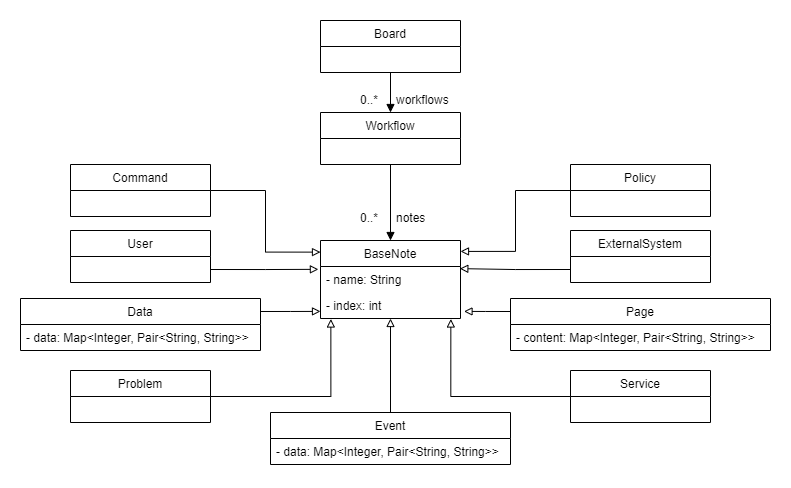
\includegraphics[width=1\textwidth]{images/3.1/classdiagram.drawio}
    \caption{Klassendiagramm fulibWorkflows}
    \label{fig:classdiagram}
\end{figure}

Bevor anhand eines Beispiels die Verwendung einer exit-Methode erläutert wird, ist es notwendig das Datenmodell genauer zu betrachten.
In Abbildung~\ref{fig:classdiagram} ist das Klassendiagramm abgebildet, welches die Struktur eines \ac{ES}-Boards nach dem Parsen der YAML-Eingabe widerspiegelt.
Jeder Note besitzt eine dazugehörige Klasse, welche von BaseNote erbt.
Für jeden Note existiert somit ein Name und ein Index, auf welchen im folgenden Abschnitt eingegangen wird.
Da es im Event Storming ein dazugehöriges \textit{Board} gibt, ist dies ebenfalls eine Klasse, welche alle \textit{workflows} einer Eingabe hält.
Ein Workflow besteht weiterhin aus vielen Notes.
Wie zuvor bereits erläutert, sind Data, Event und Page Sonderfälle unter den Notes, da diese weitere Daten beherbergen.
Daher haben diese Klassen ein Attribut, welches diese Daten organisiert in einer Map hält.
Hierbei wird als key der Index eines Notes verwendet und das value ist ein Pair.
Das Pair beinhaltet den Bezeichner und den dazugehörigen Wert einer zusätzlichen Property eines Notes.

\begin{listing}[!ht]
    \inputminted[firstnumber=106]{java}{listings/3.1.3/ExitPage.java}
    \caption{exitPage-Methode}
    \label{listing:exitpage}
\end{listing}

In Listing~\ref{listing:exitpage} wird ein neues Page-Objekt erstellt.
Bevor jedoch die exitPage-Methode aufgerufen wird, werden alle Elemente der Page in der Variable \textit{noteData} gespeichert.
Diese Elemente werden in der exitElement-Methode hinzugefügt, der Name einer Page wird hingegen in der gesonderten exitPageName-Methode zu \textit{noteData} hinzugefügt.
Zusätzlich zu den Daten eines Notes, wird diesem ein Index gegeben und anschließend zur Liste aller Notes hinzugefügt.
Der Index ist notwendig, um die Reihenfolge von Notes und deren Attributen beizubehalten.


\subsection{Generierung von Dateien}\label{subsec:generierung-von-dateien}
Aus einer workflow beschreibung können bis zu fünf verschiedene Typen von Dateien generiert werden.
Der Einstiegspunkt und somit der Start des Parsens und der Generierung ist die \textit{BoardGenerator}-Klasse.
Diese hat Methoden um Eingaben entweder von einer Datei oder eines Strings weiterzuverarbeiten.
Nachdem mittels des Parsers aus der Eingabe ein fertiges Board-Objekt erstellt wurde, werden weitere Klassen zur Generierung verwendet.
HTML-Dateien werden vom HtmlGenerator generiert, hierbei handelt es sich um Mockups und das Event Storming Board.
Mockups können allerdings auch als FXML-Datei generiert werden, um eine Grundlage für eine JavaFx-Anwendung zu bilden, diese Generierung
übernimmt der FxmlGenerator.
Zuletzt vereint der DiagramGenerator die Generierung von Objekt- und Klassendiagrammen.
Außer der \textit{BoardGenerator}-Klasse sind die restlichen Generator-Klassen für die Vorbereitung der Daten zuständig.
Diese erhalten Eingaben von dem BoardGenerator, bereiten diese Eingabe auf, je nachdem welche Daten benötigt werden und enthalten eine
separate Methode zum Erstellen von Dateien im Dateisystem.
Das Bauen einer Datei in Form eines Strings wird in einer gesonderten \textit{Constructor}-Klasse erledigt.
Da es fünf verschiedene Typen von Dateien gibt und das Bauen für jede Datei anders ist, existieren fünf \textit{Constructor}-Klassen, für jeden Dateityp eine.
Im Folgenden werden die Aufbereitungsschritte genauer beleuchtet.

\subsubsection{Event Storming Board}
Für die Generierung des Event Storming Boards bedarf es keiner Bearbeitung des HtmlGenerators, da das gesamte Board generiert werden soll und die Daten,
welche vom Parser erstellt wurden bereits optimiert sind.
Die HTML-Datei wird mittels StringTemplates, welche in einer StringTemplateGroup organisiert sind, zusammengebaut.
Für jeden workflow im Board-Objekt wird eine neue Reihe in der HTML-Datei angelegt.
Innerhalb einer workflow-Reihe werden alle dazugehörigen Notes gebaut.
Hierbei wird zwischen den verschiedenen Notes unterschieden, um verschiedene Darstellungen zu ermöglichen.
Je nach Note wird eines von drei StringTemplates verwendet.
Für die Standard-Notes wird lediglich eine neue \textit{Card}, eine Bootstrap CSS-Klasse, erstellt, welche den Typen des Notes, dessen Content und eine bestimmte Farbe übergeben bekommt.
Für die organisatorischen Notes, User, Service und ExternalSystem wird eine Card erstellt, welche kleiner als die eines normalen Notes ist.
Zudem wird in organisatorischen Notes nur ein Icon und der Bezeichner angezeigt, wobei das Icon ein Bootstrap Icon ist.
Data- und Page-Notes werden gesondert mit einem dritten StringTemplate behandelt, da es neben Typ, Content und Farbe noch einen Link gibt, welcher als Button definiert und für die Verwendung
im WebEditor genutzt wird.

\begin{figure}[h]
    \centering
    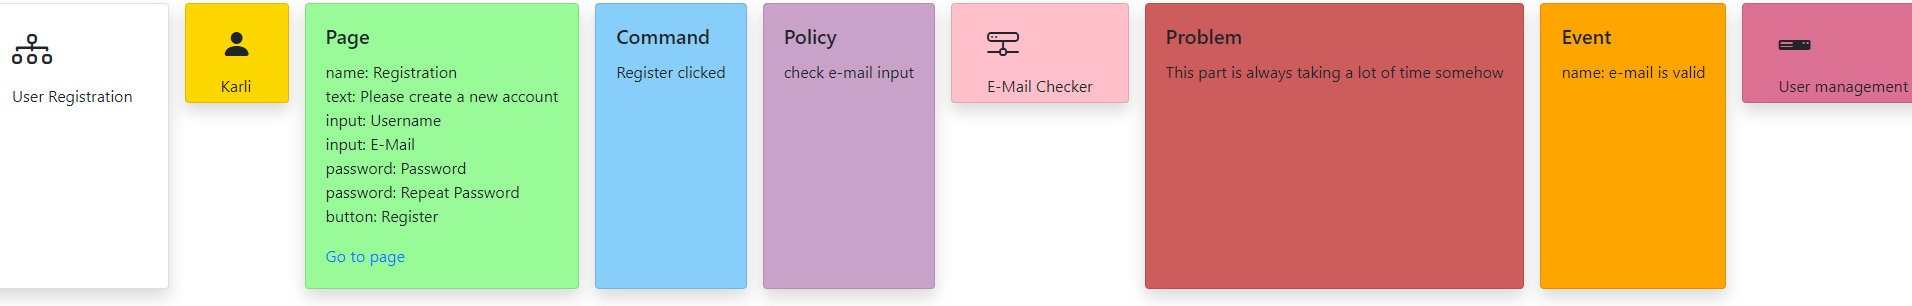
\includegraphics[width=1.0\textwidth]{images/3.1/board}
    \caption{Mittels fulibWorkflows generiertes Event Storming Board}
    \label{fig:generated-board}
\end{figure}

In Abbildung~\ref{fig:generated-board} ist ein Ausschnitt des in Listing~\ref{listing:workflowNotes} beschriebenen Workflows in
Form eines generierten Event Storming Boards dargestellt.
Hierbei sind die zuvor beschriebenen Unterschiede zwischen den verschiedenen Notes erkennbar.
Jeder Note-Typ besitzt eine eigene Farbe, wobei für User, Service und ExternalSystem eine kleinere Card und jeweils ein
eigenes Icon erkennbar sind.
Ebenfalls ist der Page-Note der Note mit den meisten Informationen in diesem Ausschnitt, da nur dort zusätzliche Informationen
in der Workflowbeschreibung existierten.

\subsubsection{Mockups HTML/FXML}
Die Generierung von HTML-Mockups wird durch die zuvor bereits erwähnte \textit{HtmlGenerator}-Klasse übernommen.
Diese filtert aus allen Workflows und den dazugehörigen Notes die Pages heraus und übergibt diese an die \textit{PageConstructor}-Klasse.
FXML-Mockups erhalten eine gesonderte Generator- und Constructor-Klasse.
Die in diesen Klassen befindlichen Funktionen ähneln der Funktionsweise des HtmlGenerators und des PageKonstruktors stark.
Eine Unterscheidung in HTML und FXML wurde lediglich vorgenommen, um bei der Generierung die Möglichkeit von verschiedenen Option offenzulassen.
Somit könnten nur HTML- oder FXML-Mockups erstellt werden.
Der FxmlConstructor und PageConstructor haben somit sowohl eine ähnliche Funktionsweise als auch einen ähnlichen Aufbau, da die zugrundeliegenden Daten die gleichen sind.
Lediglich die zugrunde liegende~\ac{STG} unterscheidet die beiden Klassen.
In beiden~\ac{STG}s gibt es ein~\ac{ST} zum Aufbau der generellen Struktur der jeweiligen Datei und für jedes verfügbare Oberflächenelement ein weiteres~\ac{ST}.
Es existieren somit für die Oberflächenelemente~\ac{ST}s für Text, Eingabefeld, Passwortfeld und Knopf.

\begin{figure}%
    \centering
    \subfloat[\centering FXML Mockup]{{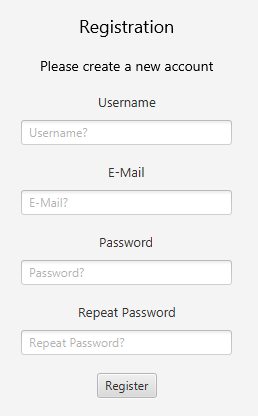
\includegraphics[width=4cm,height=6cm]{images/3.1.4/fxml-mockup} }}%
    \qquad
    \subfloat[\centering HTML Mockup]{{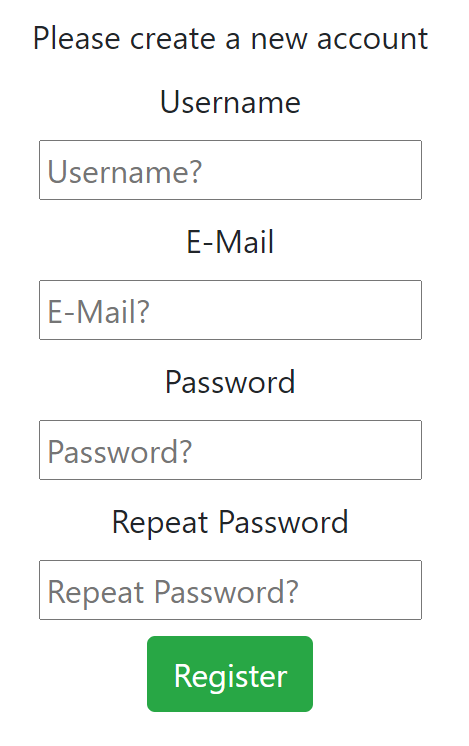
\includegraphics[width=4cm,height=6cm]{images/3.1.4/html-mockup} }}%
    \caption{Mittels fulibWorkflows generierte Mockups}%
    \label{fig:mockups}%
\end{figure}

In Abbildung~\ref{fig:mockups} sind die generierten Mockups aus dem vorherigen Beispiel dargestellt.
Diese bestehen, entsprechend der Beschreibung, aus einem Text, drei Eingabefeldern, einem Passwortfeld und einem Knopf.
Bei der Generierung wird vor allem darauf geachtet, dass sich die Oberflächen möglichst stark ähneln.
Der Aufbau der in Abbildung~\ref{fig:mockups}((a)) und Abbildung~\ref{fig:mockups}((b)) Oberflächen ist somit identisch, Unterschiede
sind lediglich durch das Stylen des HTML-Mockups, mittels Bootstrap, zu erkennen.

\subsubsection{Objektdiagramme}
Zuletzt gibt es die \textit{DiagramGenerator}-Klasse, welche die Eingabe für Objekt- und Klassendiagramme aufarbeitet.
Jeder Data-Note erhält sein eigenes Objektdiagramm.
Damit die zeitliche Abfolge und somit ein korrektes Objektdiagramm entsteht, wird jeder Data Note zu einer Liste hinzugefügt und diese anschließend an die
\textit{ObjectDiagramConstructor}-Klasse übergeben.
Hierdurch werden pro Data Note mehr Objekte zu dem dazugehörigen Objektdiagramm hinzugefügt, sollte es eine Verbindung zu einem bestehenden Objekt geben.
FulibTools verwendet Graphviz zur Erstellung von Diagrammen, zusätzlich besitzt FulibTools die Möglichkeit Objekt- und Klassendiagramme anhand einer bestimmten Eingabe zu generieren.
Diese Funktionalität macht sich fulibWorkflows im ObjectDiagramConstructor zunutze.
Aus der übergebenen Liste an Data Notes baut der ObjectDiagramConstructor eine YAML-Datei, welche den Spezifikationen von fulibYaml entspricht.
In Listing~\ref{listing:fulibYaml} ist die zum ObjectDiagramConstructor gehörende \ac{STG}-Datei abgebildet.
Ein Objekt benötigt immer einen Namen, eine Klasse in Zeile 5 als \textit{type} gekennzeichnet und optionale Attribute.
Die Form eines Attributes ist in dem \ac{ST} ab Zeile 10 abgebildet, ein Attribute besteht lediglich aus einer Klasse, erneut \textit{type} genannt, und dem
dazugehörigen Wert.

\begin{listing}[!ht]
    \inputminted[xleftmargin=20pt,linenos]{text}{listings/3.1.4/FulibYaml.stg}
    \caption{FulibYaml.stg}
    \label{listing:fulibYaml}
\end{listing}

Nachdem ein Objektdiagramm in fulibYaml Notation vorhanden ist, wird FulibTools verwendet um daraus ein Diagram zu generieren.
In Listing~\ref{listing:object-gen} ist diese Generierungsmethode abgebildet.
Der erste Parameter der Methode enthält die Objektstruktur in Form von fulibYaml als String.
Daraus wird in Zeile 99 und 100 ein root-Objekt erstellt, welches die Klasse \textit{YamlIdMap} aus der Bibliothek fulibYaml nutzt.
Dieses root-Objekt wird gemeinsam mit dem in Zeile 96 festgelegten Dateinamen durch FulibTools in Zeile 102 generiert.
FulibTools erlaubt bei der Generierung nicht, dass der Inhalt der zu generierenden Datei zurückgegeben wird, die Datei wird sofort im Dateisystem erstellt.

\begin{listing}[!ht]
    \inputminted[xleftmargin=20pt,linenos,firstnumber=95]{java}{listings/3.1.4/ObjectGeneration.java}
    \caption{Generierungsmethode eines Objektdiagramms}
    \label{listing:object-gen}
\end{listing}

Im Anschluss an die Generierung durch FulibTools wird der Inhalt der generierten Datei als String ausgelesen und von der Methode zurückgegeben.
Danach wird die generierte Datei, sowie ein Ordner wieder gelöscht.
Dies hat den Hintergrund, dass die Generierung von Dateien, in Form vom Speichern im lokalen Dateisystem, gesammelt in der BoardGenerator-Klasse vollzogen werden soll.
Zudem wird im BoardGenerator die Möglichkeit geboten, Dateien aus einer Workflow Beschreibung zu generieren und diese als String zurückzugeben.
Diese Methoden existieren für die Nutzung im fulibWorkflows Web-Editor, später dazu mehr.

\subsubsection{Klassendiagramme}
\todo{Wie wird aus allen Objekten ein Klassendiagramm? Aufbauen eine neuen Klassenmodells mittels fulib und dann fulibtools zur generierung mit Bildern}



\section{Frontend des Web-Editors}\label{sec:editor-frontend}
Nachdem die erste Hälfte der Implementierung durch fulibWorkflows abgeschlossen ist, konzentrieren sich dieses und das folgende Kapitel um den dazugehörigen Web-Editor.
Der Web-Editor besteht aus einem Frontend und einem Backend, welche beide über Heroku deployt wurden und somit\footnote{unter \url{https://workflows-editor-frontend.herokuapp.com/}}
erreichbar sind.

\begin{figure}[h]
    \centering
    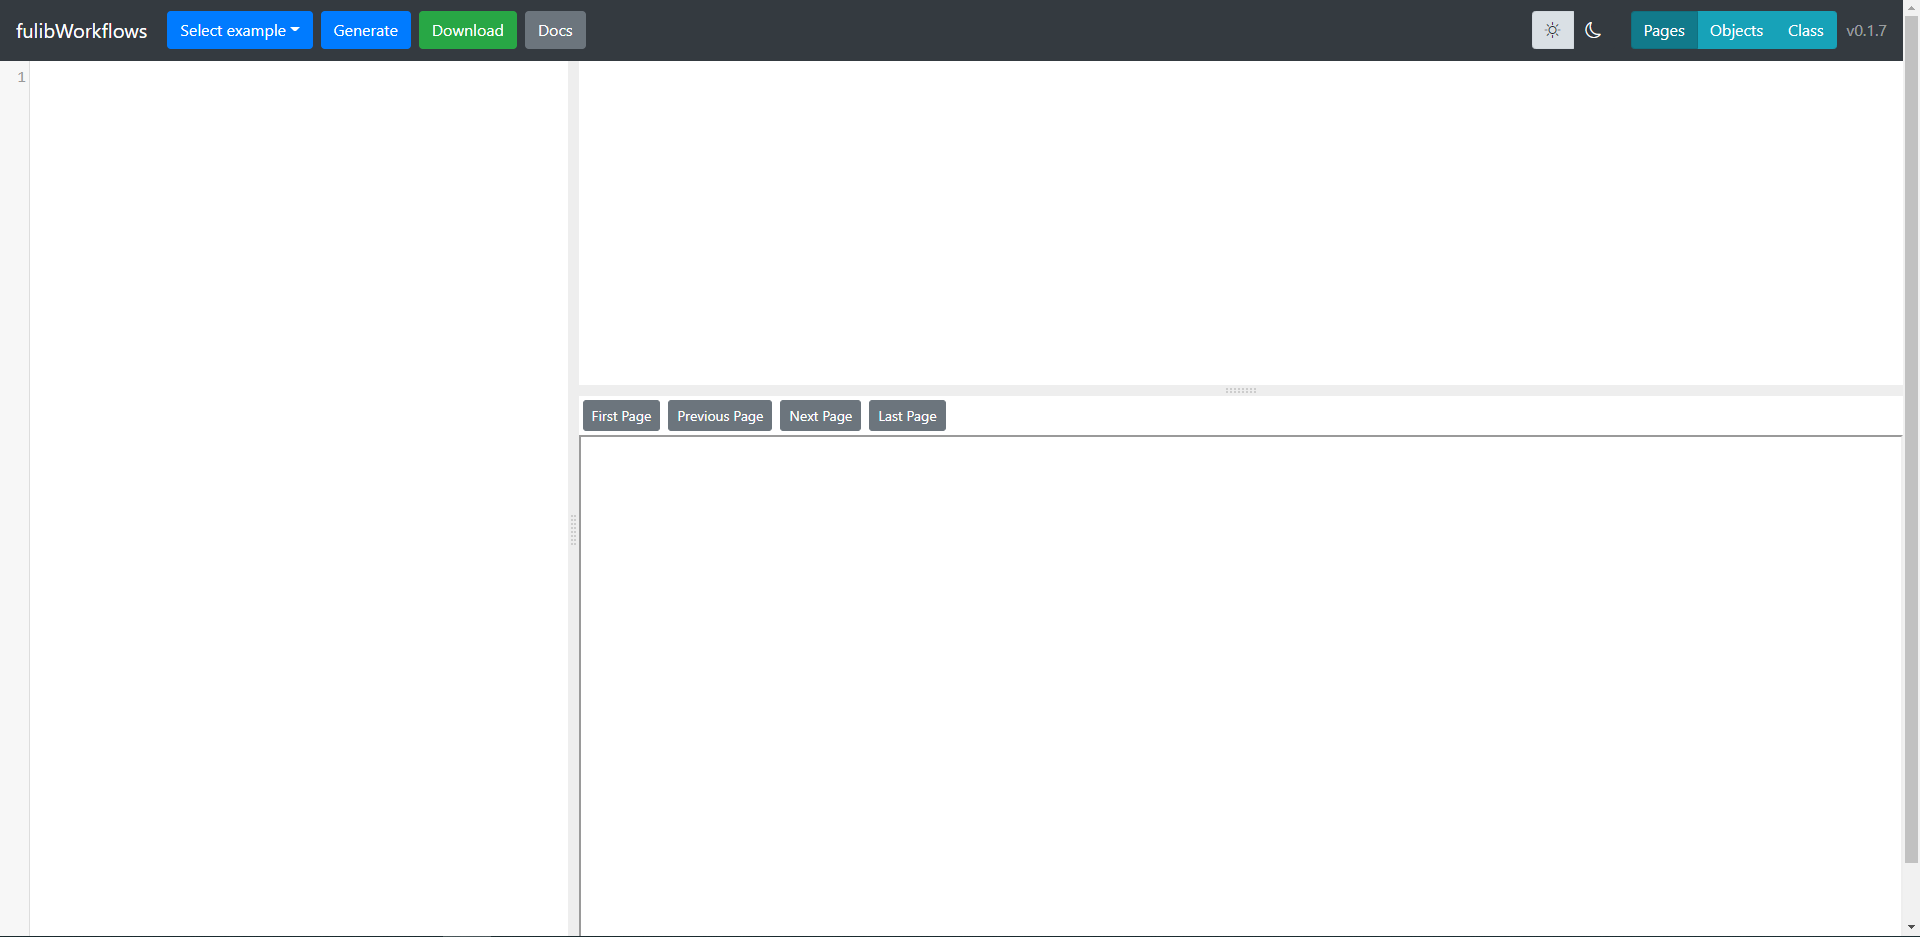
\includegraphics[width=1.0\textwidth]{images/3.2/workflows-complete}
    \caption{Oberfläche des Web-Editors für fulibWorkflows}
    \label{fig:frontend}
\end{figure}

In Abbildung~\ref{fig:frontend} ist die Oberfläche des Web-Editors dargestellt.
Dieser besteht aus vier verschiedenen Bereichen.
Der erste dieser Bereiche ist die Navigationsleiste, welche den oberen Rand der Oberfläche einnimmt.
In dieser existieren zuerst, von links nach rechts, zwei Buttons, welche das Theme des Code-Editors abändern.
Damit ist es möglich einen Light- oder Dark-Mode zum Schreiben des Codes zu verwenden.
Danach folgt ein Dropdown-Menü, mit welchem es möglich ist verschiedene vorgefertigte Beispiele zu laden.
Das ausgewählte Beispiel wird automatisiert nach der Auswahl ans Backend geschickt und dort generiert, sodass nach einer kurzen Wartezeit ein \ac{ES}-Board und falls
vorhanden Mockups und Diagramme angezeigt werden können.
Als Nächstes folgt ein Knopf zum Anstoßen einer Generierung, nachdem dieser Knopf gedrückt wurde und die Generierung angestoßen ist, erscheint ein Ladekreis in dem Knopf,
um als Indikator dafür zu dienen, dass der Prozess noch nicht abgeschlossen ist.
Die Web-Anwendung ermöglicht es zusätzlich die in der Oberfläche erstellten Dateien herunterladen.
Hierfür öffnet sich ein Pop-Up, nachdem der Download-Knopf betätigt wurde.
Dieses Fenster ist in Abbildung~\ref{fig:download} dargestellt.

\begin{figure}[h]
    \centering
    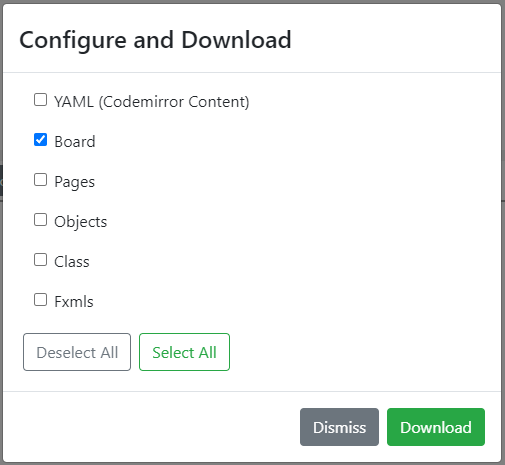
\includegraphics[width=0.5\textwidth]{images/3.2/download}
    \caption{Download-Fenster}
    \label{fig:download}
\end{figure}

Im sich öffnenden Fenster erhält der Benutzende die Möglichkeit auszuwählen, welche Dateien heruntergeladen werden sollen.
Es können einzelne Dateien heruntergeladen werden, wie der Inhalt des Code-Editors, das generierte \ac{ES}-Board oder aber alle Dateien
die durch die aktuelle Workflow-Beschreibung im Code-Editor generiert wurden.
Mit einem Klick auf den Download-Knopf, welcher sich neben dem Dismiss-Knopf befindet, wird eine Zip-Datei generiert und automatisch durch den jeweiligen Browser heruntergeladen.

Für den Fall, dass der Nutzende noch keine Erfahrungen mit der Syntax von fulibWorkflows gemacht hat, kann die Dokumentation, welche auf Englisch verfasst ist, mit einem Klick
auf den grauen Docs-Knopf aus Abbildung~\ref{fig:frontend} geöffnet werden.
Die Dokumentation stammt aus dem GitHub-Repository von fulibWorkflows.
Letztlich befindet sich ganz rechts die aktuelle Versionsnummer des Web-Editors.

\subsection{Code-Editor}\label{subsec:codeeditor}
In diesem Kapitel wird der Code-Editor, welcher das Herzstück der Anwendung ist, erläutert.
Dieser befindet sich auf der linken Seite der in Abbildung~\ref{fig:frontend} dargestellten Oberfläche.
Wie zuvor bereits beschrieben wurde hierbei ein Codemirror verwendet.
Durch die Verwendung der \textit{ngx-codemirror} Bibliothek vereinfacht sich das Einbinden eines Codemirrors in eine Angular-Anwendung.
Dadurch kann eine Konfiguration des Codemirrors über ein Options-Objekt übergeben werden.
Die Konfiguration des Codemirrors ist in Listing~\ref{listing:configuration} dargestellt.

\begin{listing}[!ht]
    \inputminted[firstnumber=49]{ts}{listings/3.2/codemirror-options.ts}
    \caption{Codemirror-Konfiguration}
    \label{listing:configuration}
\end{listing}

In Zeile 50 werden die Zeilennummern am linken Rand des Codemirrors aktiviert.
Das aktuelle Theme wird in der folgenden Zeile ebenfalls übergeben.
Da es zwei verschiedene Themes gibt, welche verwendet werden können, wird der Wert aus einer weiteren Variable übernommen.
Codemirror stellt bereits zahlreiche verschiedene Themes für Light-Mode oder Dark-Mode bereit.
Initial wird der Codemirror mit dem Light-Theme geladen, das Umstellen des Themes erfolgt über die entsprechenden Knöpfe in der Navigationsleiste, wie bereits zuvor beschrieben.
Abbildung~\ref{fig:themes} zeigt den Codemirror in beiden Modi, wobei sich sowohl Light- als auch Dark-Mode nah an den Standard-Modi von IntelliJ orientieren.

% Diese Abbildungen ggf. in den Anhang verschieben
\begin{figure}%
    \centering
    \subfloat[\centering Light-Theme]{{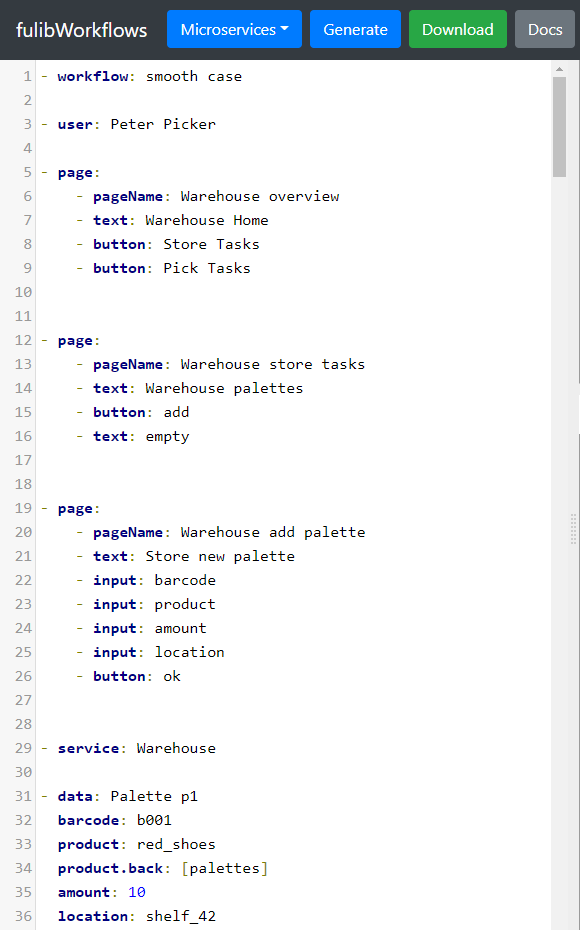
\includegraphics[width=4cm,height=6cm]{images/3.2/light-theme} }}%
    \qquad
    \subfloat[\centering Dark-Theme]{{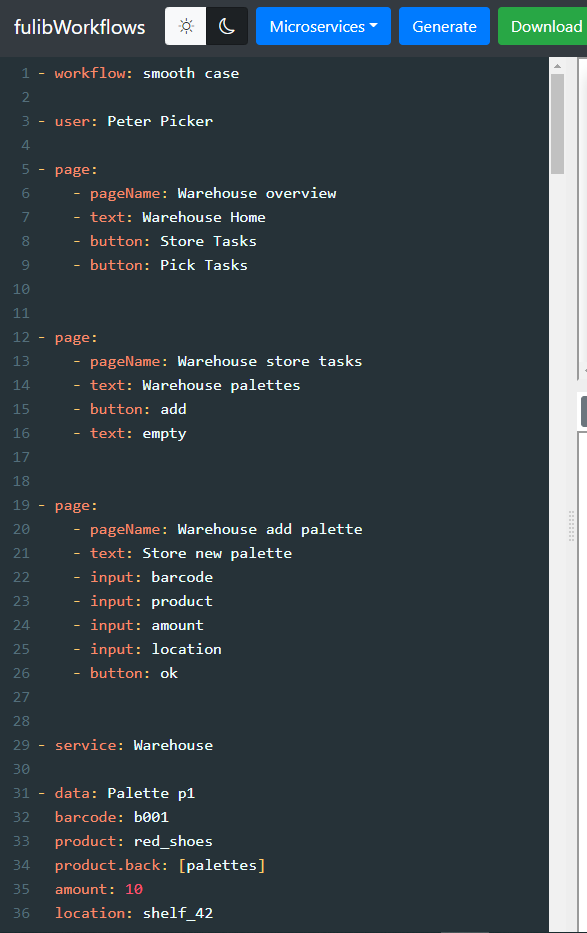
\includegraphics[width=4cm,height=6cm]{images/3.2/dark-theme} }}%
    \caption{Themes des Codemirrors}%
    \label{fig:themes}%
\end{figure}

In Zeile 52 aus Listing~\ref{listing:configuration} wird die Programmiersprache des Editors festgelegt.
Da die Workflow-Beschreibungen von fulibWorkflows in \textit{.es.yaml}-Dateien angelegt/gespeichert werden, wird die Programmiersprache auf \textit{yaml} festgelegt.
Dieser Modus wird von Codemirror selbst bereitgestellt und bedarf zur Verwendung lediglich eines Importes in der \textit{main.ts}-Datei der Angular-Anwendung.
Über die Option \textit{extraKeys} können Tasten oder Tastenkombinationen an weitere Funktionen gekoppelt werden.
In Zeile 54 wird das Öffnen einer Liste an vorgeschlagenen Wörtern geöffnet, nachdem der Nutzende die Tastenkombination ``Strg+Leertaste'' gedrückt hat.
Damit dies funktioniert, benötigt es das Importieren des \textit{show-hint}-AddOns von Codemirror in der \textit{main.ts}-Datei.

\begin{figure}%
    \centering
    \subfloat[\centering Ohne Eingabe]{{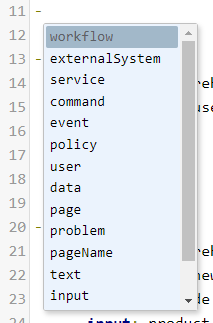
\includegraphics[width=4cm,height=6cm]{images/3.2/autocompletion-all} }}%
    \qquad
    \subfloat[\centering Mit Eingabe]{{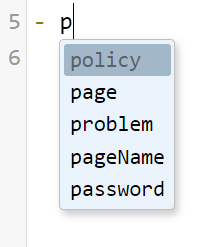
\includegraphics[width=4cm,height=5cm]{images/3.2/autocompletion-p} }}%
    \caption{Autovervollständigung}%
    \label{fig:autocompletion}%
\end{figure}

Dieses Add-On erstellt die in Abbildung~\ref{fig:autocompletion}((a)) angezeigt Liste.
Der Inhalt der Liste wird über ein in dieser Arbeit erstelltes Codemirror Add-On gefüllt.
Hierbei fällt auf, dass auch Schlüsselwörter angezeigt werden, welche nur im Kontext eines Page-Notes sinnvoll sind.
Das eigens geschriebene Add-On ist nicht kontextsensitiv und besitzt somit nicht die gleichen Funktionen wie die Autovervollständigung, welche eine IDE durch das JSON-Schema bereitstellt.
Der Code des geschriebenen Add-Ons befindet sich im Anhang dieser Arbeit, hierbei wird über die aktuelle Position des Cursors das aktuelle Wort extrahiert.
Damit ist es möglich über die Liste der Schlüsselwörter zu iterieren und zu prüfen, welche Vorschläge sinnvoll sind, sollte ein Wort bereits begonnen sein.
Dies ist anhand von Abbildung~\ref{fig:autocompletion}((b)) genauer zu erkennen.
Hierbei wurde bereits der Buchstabe \textit{p} eingetippt und das Add-On bietet zur Vervollständigung lediglich Wörter an, welche mit \textit{p} beginnen.

Des Weiteren wird durch das Betätigen der Tastenkombination ``Strg+S'' die Generierung angestoßen.
Bevor die Daten aus dem Codemirror zur Generierung an das Backend gesendet werden, werden diese auf Richtigkeit überprüft.
Da bereits ein JSON-Schema für fulibWorkflows existiert, wurde eine Bibliothek ausgewählt, welche einen Text über ein JSON-Schema validieren kann.
\textit{Ajv} ist ein solcher Validierungsmechanismus, allerdings kann mit Ajv lediglich ein JSON-Objekt mittels JSON-Schema validiert werden\cite*{ajv}.
Somit wurde zum Umwandeln des Textes aus dem Codemirror zu einem JSON-Objekt die Bibliothek \textit{js-yaml} verwendet\cite*{js-yaml}.

\begin{figure}[h]
    \centering
    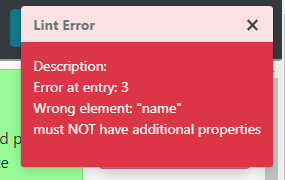
\includegraphics[width=0.4\textwidth]{images/3.2/error-toast}
    \caption{Validierungserror als Toast}
    \label{fig:error-toast}
\end{figure}

Sobald während der Validierung ein Problem mit der Eingabe erkannt wird, gibt diese einen Fehler zurück.
Dieser Fehler wird anschließend als Toast in der Oberfläche angezeigt, um den Nutzenden darauf hinzuweisen, an welcher Stelle die Eingabe im Codemirror nicht
dem JSON-Schema von fulibWorkflows entspricht.
Eine solche Fehlermeldung ist in Abbildung~\ref{fig:error-toast} dargestellt.
Hierbei wurde einem Note ein Attribut \textit{name} zugeordnet.
Da der besagte Note allerdings ein \textit{User} ist und im JSON-Schema festgelegt ist, dass ein User-Note keine zusätzlichen Attribute
besitzen darf, entsteht der in der Abbildung gezeigte Fehler.
Diese Fehlermeldung wird nach 20 Sekunden automatisch geschlossen.
Für die Darstellung von Toasts wurde die gleichnamige Komponente von \textit{ng-bootstrap} verwendet.
Sollte die Eingabe valide sein, so wird diese über einen Service an das Backend geschickt.

\subsection{Darstellung generierter Dateien}\label{subsec:darstellung-generierter-dateien}
Die anderen beiden Bereiche der Oberfläche, welche bisher nicht erläutert wurden, stellen jeweils einen bestimmten Teil der generierten Dateien dar.
Beide Bereiche aus Abbildung~\ref{fig:frontend} bestehen aus einem IFrame, wobei der obere IFrame lediglich das generierte \ac{ES}-Board anzeigt.
Andererseits übernimmt der untere IFrame die Anzeige der HTML-Mockups, den Objektdiagrammen und dem Klassendiagramm.

\begin{listing}[!ht]
    \inputminted{ts}{listings/3.2/GenerateResult.ts}
    \caption{Modell der vom Backend empfangenen Daten}
    \label{listing:generateResult}
\end{listing}

Bevor auf die Darstellung und Funktionen der IFrames eingegangen wird, wird zuerst betrachtet in welcher Form die generierten Dateien vom Backend im Frontend verarbeitet werden.
Die Form ist in Listing~\ref{listing:generateResult} dargestellt, in einem GenerateResult-Objekt werden alle generierten Dateien und Zusatzinformationen abgespeichert.
Bei den Zusatzinformationen handelt es sich um die Anzahl der generierten Diagramme und HTML-Mockups.
Die generierten Dateien werden lediglich als reiner String behandelt.
Um den Zugriff auf einzelne Objektdiagramme oder Mockups zu vereinfachen, sind diese jeweils in einer Map abgespeichert.
Bei den Maps ist jedem Diagramm/Mockup eine eindeutige Nummer zugeordnet.

Der obere IFrame erhält als Eingabe das \ac{ES}-Board und stellt dieses dar.
Dies ist möglich, da das \ac{ES}-Board eine valide HTML-Datei ist, welche durch einen IFrame dargestellt werden kann.
Hierbei war es nötig eine Pipe zu erstellen, welche den \textit{DomSanitizer} von Angular auf der Eingabe umgeht\cite*{safe-pipe}.
Der DomSanitizer ist ein von Angular bereitgestellter Service, welcher Elemente aus der Eingabe entfernt die potenziell für Angreifer genutzt werden könnten, um
Skripte auf der Anwendung auszuführen.
Dies ist ein Sicherheitsmechanismus, um das sogenannte \textit{Cross-Site-Scripting} auszuhebeln.
Beim \textit{Cross-Site-Scripting} können Angreifer JavaScript-Code in den Browsern anderer Nutzer ausführen und somit personenbezogene Daten erhalten\cite*{xss}.
Durch die Pipe wird dieser Sicherheitsmechanismus umgangen und die Eingabe wird unverändert im IFrame geladen.

\todo{Heißt das, dass die Anwendung jetzt angegriffen werden kann? Das wär ja blöd oder? -> Ja das heißt es. Lösungsansatz im Ausblick beschreiben und darauf hier verweisen}

\begin{figure}[h]
    \centering
    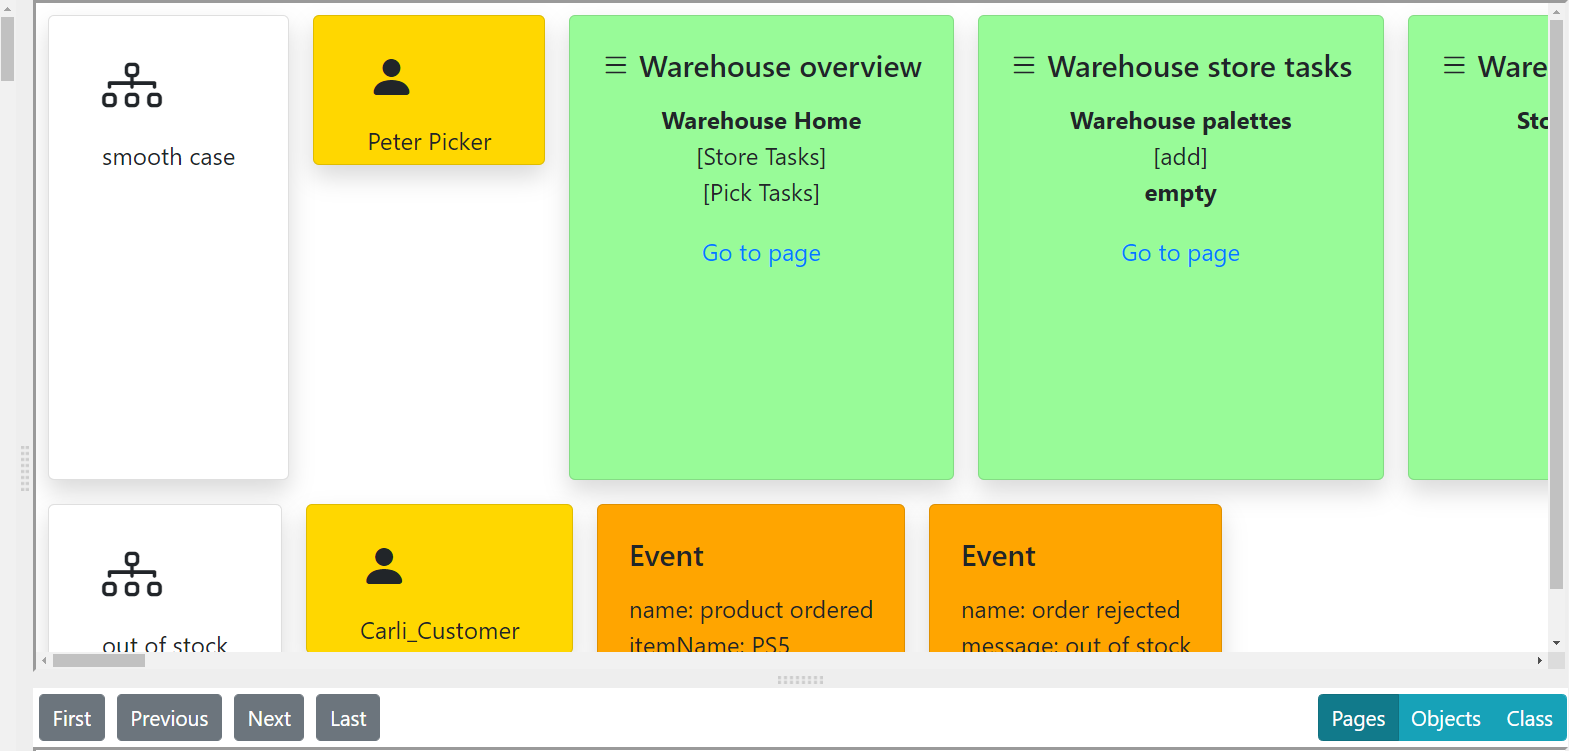
\includegraphics[width=1.0\textwidth]{images/3.2/board}
    \caption{Event-Storming-Board in einem IFrame}
    \label{fig:esBoard}
\end{figure}

In Abbildung~\ref{fig:esBoard} ist ein Event-Storming-Board für das im Web-Editor vorhandene Microservices-Beispiel dargestellt.
Hierbei ist zu erwähnen, dass die Bereiche: Code-Editor, \ac{ES}-Board-IFrame und der IFrame zur Anzeige der Mockups und Diagramme beliebig vergrößert oder verkleinert werden kann.
Um dies zu ermöglichen wurde die Bibliothek \textit{angular-split} verwendet.
Diese ermöglicht es Bereiche zu definieren und darin Inhalt zu platzieren, sowie die Veränderung der Größen der Bereiche bereitzustellen\cite*{angular-split}.
Das Abändern der Größe von Bereichen ermöglicht das Hervorheben des Editors, des \ac{ES}-Boards oder der Mockups/Diagramme.

Für den unteren IFrame gelten die gleichen Gegebenheiten wie für den oberen IFrame.
Da es mehrere Mockups oder Diagramme geben kann, existieren vier Knöpfe, mit welchen es möglich ist zwischen den Mockups/Diagrammen zu wechseln.
Doch der Wechsel zwischen diesen Elementen ist nicht nur über die vier Knöpfe möglich, sondern ebenfalls über die entsprechenden Notes aus dem \ac{ES}-Board-IFrame.
Für jeden Page- oder Data-Note existiert in der Anzeige ein Link, welcher als Knopf fungiert, mit welchem zu dem Mockup oder Diagramm des Notes gewechselt werden kann.

\begin{listing}[!ht]
    \inputminted{ts}{listings/3.2/method.ts}
    \caption{Bereitstellung einer Methode}
    \label{listing:global-method}
\end{listing}

Hierfür ist eine Methode erstellt worden, welche für die gesamte Oberfläche sichtbar ist.
In der Generierung mittels fulibWorkflows wird dieser Link erstellt, darin wird die bereitgestellte Methode mittels~\texttt{window.parent.setIndexFromIframe(0, `pages');} aufgerufen.
\todo{hmmm vielleicht auch ein snippet zur erklärung einfügen, statt das direkt in den text zu schreiben?}
Hierbei wird über das Fenster auf die oberste Komponente der Anwendung zugegriffen, dort ist durch den Code aus Listing~\ref{listing:global-method}
die Methode \textit{setIndexFromIframe} bereitgestellt.
Neben dem Index wird der Methode ebenfalls ein String übergeben, mit diesem ist es möglich zwischen Page und Object-Darstellung automatisch beim Klicken des Links zu wechseln.

\todo{so generell zu diesem absatz... ist das sehr wichtig? dann vielleicht ausführlicher erklären... wenn unwichtig.. vielleicht weglassen? kA also ich wurde da jetzt nicht so richtig schlau draus beim lesen}

Zuletzt existieren drei weitere Buttons auf Höhe der Buttons zum Wechseln der Page oder des Diagramms, welche die Anzeige der generierten Dateien manuell umschaltet.
\todo{ja wo denn ich seh nix}
Hierbei kann zwischen dem Anzeigen der Mockups (Pages), der Objektdiagramme und des Klassendiagramms umgeschaltet werden.


\section{fulibWorkflows Web-Editor Backend}\label{sec:editor-backend}
Das Backend des Web-Editors basiert auf einem mit Spring Initializr generiertem Java Projekt.
Zusätzlich wurden bei der Konfiguration die Dependencies für eine Spring Web Anwendung hinzugefügt.
Neben den eben genannten Dependencies wurde lediglich fulibWorkflows als weitere Bibliothek zum Backend hinzugefügt.

Die verfügbaren Endpunkte des Backends werden in einem Controller bereitgestellt.
In diesem fall ist dies der FulibWorkflowsController, welcher mit zwei Annotations versehen ist.
Die erste Annotation ist~\texttt{@Controller}, welche der Anwendung mitteilt, dass diese Klasse als Controller agiert.
Bei der zweiten Annotation handelt es sich um \texttt{@CrossOrigin()} mit welcher es ermöglicht wird problemlos mit dem
Frontend zu interagieren.
Im FulibWorkflowsController sind Endpunkte für die Generierung und den Download definiert.
Diese Definitionen werden in Listing~\ref{listing:endpoints} zur Veranschaulichung dargestellt.

\begin{listing}[!ht]
    \inputminted[xleftmargin=20pt,linenos,firstnumber=15]{java}{listings/3.3/Endpoints.java}
    \caption{Definition der Endpunkte}
    \label{listing:endpoints}
\end{listing}

Beide Endpunkte können mit einem POST-Request angesprochen werden, da sowohl beim Download als auch der Generierung der Inhalt der
yaml Datei vom Frontend mitgeschickt wird.
Dies sorgt dafür, dass bei beiden Endpunkten die Generierung durchgeführt wird, um kein Abspeichern von Dateien und Vergabe von IDs für
eine Beschreibung angelegt und verwaltet werden muss.
Damit die Endpunkte auf diesen Inhalt zugreifen können, ist der erste Methodenparameter mit der \texttt{@RequestBody} Annotation versehen.
Hierbei wird auf den Inhalt zugegriffen, welcher vom Frontend in der Post-Anfrage mitgesendet wurde.
Der Downlaod-Endpunkt erhält zusätzlich zu der yaml Beschreibung ebenfalls Query-Parameter.
Diese enthalten die aus dem Download-PopUp des Frontends angegeben Dateien, welche heruntergeladen werden sollen.
Mittels der \texttt{@ResponseBody} Annotation, können der Antwort des Backends weitere Daten hinzugefügt werden, in welcher Form diese
sind, resultiert aus dem Rückgabetyp der jeweiligen Methode unterhalb der Annotation.
Bei der Generate-Methode wird ein JSON-Objekt als String zurückgegeben, wobei bei der Download-Methode das generierte Zip-Archiv als ByteArray verwendet wird.
Beide Methoden des Controllers reichen die erhaltenen Daten an den FulibWorkflowsService weiter, welcher sich um die Generierung über fulibWorkflows
und der Erstellung des Zip-Archives kümmert.

Im FulibWorkflowsService, wird sowohl in der generate- als auch der createZip-Methode, welche vom Controller aufgerufen werden,
der yaml-String über fulibWorkflows generiert.
Dabei nutzt das Backend die \texttt{generateAndReturnHTMLsFromString}-Methode des BoardGenerators von fulibWorkflows.
Im Anschluss wird aus der Map von generierten Dateien ein GenerateResult erstellt, welches von der generate-Methode zu einem JSON-String weiterverarbeitet und zurück an den Controller gibt.
Nachdem das GenerateResult-Objekt in der createZip-Methode erstellt wurde, beginnt das Erstellen des Zip-Archivs.
Auf Grundlage der Query-Parameter werden lediglich die Dateien zum Zip-Archiv hinzugefügt, welche im Frontend ausgewählt werden.
In Abbildung~\ref{fig:export} sollen alle Dateien heruntergeladen werden, welche von fulibWorkflows generiert wurden.

\begin{figure}[h]
    \centering
    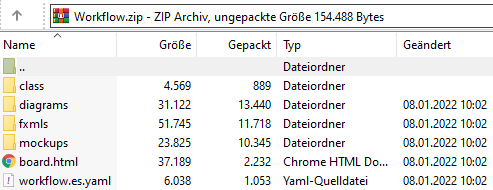
\includegraphics[width=0.6\textwidth]{images/3.3/export}
    \caption{Inhalt eines heruntergeladenen Zip-Archivs}
    \label{fig:export}
\end{figure}

Um die Dateien strukturiert zu halten, werden Diagramme und Mockups in eigenen Unterordner abgelegt.
Hierbei wird zwischen Objektdiagrammen und dem Klassendiagramm, als auch zwischen HTML- und FXML-Mockups unterschieden.
Auf oberster Ebene werden sowohl die Workflowbeschreibung als auch das generierte Event Storming Board abgelegt, da diese
die Grundlage für alle weiteren Dateien legen.
Das Klassendiagramm ist im Ordner \textit{class} abgelegt, die Objektdiagramme im \textit{diagrams}-Ordner.
Im Gegensatz hierzu, werden die HTML-Mockups im \textit{mockups}-Ordner hinterlegt, die gleichen Mockups im FXML-Format werden
im \textit{fxmls}-Ordner platziert.


\chapter{Evaluation}\label{ch:evaluation}
In diesem Kapitel wird mittels eines Expertengespräches eine Einschätzung über die Erfüllung der in
Kapitel~\ref{sec:ziele} definierten Ziele eingeholt.
Weiterhin sollte durch das Durchgehen der vorhandenen Beispiele aus der erstellten Anwendung Probleme und/oder weitere
Funktionen erkannt werden.

\section{Expertengespräch}\label{sec:expertengespraech}
\todo{THE}

\todo{I have no freakin' idea}


\chapter{Fazit}\label{ch:fazit}
\todo{Machen die Erweiterungen Sinn?}

\todo{Kann der Editor von Leuten verwendet werden, die nur wenig Programmiererfahrung haben?}

\todo{Füllt diese Anwendung eine bestehende Lücke im RE?}

\todo{Wurde das zuvor gesetzte Ziel erreicht?}

\todo{Falls nein, kann auf der Grundlage dieser Arbeit etwas Besseres geschaffen werden?}

\chapter{Ausblick}\label{ch:ausblick}
\todo{Einbindung des Web-Editors in fulib.org}

fulib.org sammelplattform für alle fulib bezüglichen Bestandteile -> Alles der fujaba tool suite an einem ort

\todo{Verwendung des Tools in der Lehre des Fachgebiets}

\todo{Erweiterungen die mir aufgefallen sind}

\todo{Erweiterungen von Adam und anderen}


\printbibliography[title={Quellenverzeichnis}]

\end{document}
